% !TEX root
% !TEX program = xelatex
% !BIB program = biber

% \def \PrintMode{} %在使用电子版论文时,请将此行注释。在打印纸质论文时,请保持本行命令不被注释,然后打印时选择双面打印即可。

%用来控制是否启动打印模式的宏,请勿改动。
\ifx \PrintMode \undefined
    \def \SideMode{oneside}
    \def \ClearPageStyle{\clearpage}
\else
    \def \SideMode{twoside}
    \def \ClearPageStyle{\cleardoublepage}
\fi

\documentclass[a4paper,oneside,UTF8]{article} %A4纸,单面,UTF-8

\usepackage[thmmarks,hyperref]{ntheorem} %定义命令环境使用的宏包
\usepackage[heading]{ctex} %用来提供中文支持
\usepackage{amsmath,amssymb} %数学符号等相关宏包
\usepackage{graphicx} %插入图片所需宏包
\usepackage{xspace} %提供一些好用的空格命令
\usepackage{tikz-cd} %画交换图需要的宏包
\usepackage{url} %更好的超链接显示
\usepackage{array,booktabs} %表格相关的宏包
\usepackage{ccaption} %实现图片的多行说明
\usepackage{subfigure}
\usepackage[subfigure]{tocloft}
\usepackage{multirow}
\usepackage{float} %图片与表格的更好排版
\usepackage{ulem} %更好的下划线

\usepackage[top=2.5cm, bottom=2.0cm, left=3.0cm, right=2.0cm]{geometry} %设置页边距

\usepackage{fontspec} %设置字体需要的宏包
\usepackage{amsfonts,amssymb}
\renewcommand{\normalsize}{\zihao{-1}}  %设置正文字号为小四

%设置西文字体为Times New Roman,如果没有则以开源近似字体代替
\IfFontExistsTF{Times New Roman}{
	\setmainfont{Times New Roman}
}{
	\usepackage{newtxtext,newtxmath}
}

%设置文档中文字体。优先次序:中易 > Adobe > 华文(Mac) > Fandol
\IfFontExistsTF{SimSun}{
	\setCJKmainfont[AutoFakeBold=2,ItalicFont=KaiTi]{SimSun}
}{
	\IfFontExistsTF{AdobeSongStd-Light}{
		\setCJKmainfont[AutoFakeBold=2,ItalicFont=AdobeKaitiStd-Regular]{AdobeSongStd-Light}
	}{
		\IfFontExistsTF{STSong}{
			\setCJKmainfont[AutoFakeBold=2,BoldFont=STHeiti,ItalicFont=STKaiti]{STSong}
		}{
			\setCJKmainfont[AutoFakeBold=2,ItalicFont=FandolKai-Regular]{FandolSong-Regular}
		}
	}
}
\IfFontExistsTF{SimHei}{
	\setCJKsansfont[AutoFakeBold=2]{SimHei}
}{
	\IfFontExistsTF{AdobeHeitiStd-Regular}{
		\setCJKsansfont[AutoFakeBold=2]{AdobeHeitiStd-Regular}
	}{
		\IfFontExistsTF{STHeiti}{
			\setCJKsansfont [AutoFakeBold=2]{STHeiti}
		}{
			\setCJKsansfont[AutoFakeBold=2]{FandolHei-Regular}
		}
	}
}

\IfFileExists{zhlineskip.sty}{
	%Microsoft Word 样式的1.5倍行距(按中易字体计算)
	\usepackage[
		restoremathleading=false,
		UseMSWordMultipleLineSpacing,
		MSWordLineSpacingMultiple=1.5
	]{zhlineskip}
}{
	\linespread{1.621} %1.5倍行距
}

\showboxdepth=5
\showboxbreadth=5

%设置各级系统的编号格式
\setcounter{secnumdepth}{5}
\ctexset { section = { name={,.},number={\arabic{section}},format={ \heiti \zihao {-4}} } }
\ctexset { subsection = { name={,},number={\arabic{section}.\arabic{subsection}},format={\heiti \zihao {-4}} } }
\ctexset { subsubsection = { name={,},number={\arabic{section}.\arabic{subsection}.\arabic{subsubsection}},format={\heiti \zihao {-4}} } }
\ctexset { paragraph = { name={(,)},number={\arabic{paragraph}},format={\heiti \zihao {-4}} } }
\ctexset { subparagraph = { name={,)},number={\arabic{subparagraph}},format={\heiti \zihao {-4}} } }


\usepackage[bottom,perpage]{footmisc}               %脚注,显示在每页底部,编号按页重置
\renewcommand*{\footnotelayout}{\zihao{-5}\rmfamily}  %设置脚注为小五号宋体
\renewcommand{\thefootnote}{[\arabic{footnote}]}    %设置脚注标记为  [编号]

%设置页眉页脚
\usepackage{fancyhdr}
\lhead{华东师范大学学士学位论文(设计)}
\chead{}
\rhead{\TitleCHS}
\lfoot{}
\zihao{-5}\cfoot{\thepage}
\rfoot{}

\usepackage{xcolor} %彩色的文字

\usepackage[hidelinks]{hyperref} %各种超链接必备
\usepackage{cleveref} %交叉引用

%设置尾注
\usepackage{endnotes}
\renewcommand{\enotesize}{\zihao{5}}
\renewcommand{\notesname}{\sffamily \zihao {-4} 尾注}
\renewcommand\enoteformat{
	\raggedright
	\leftskip=1.8em
	\makebox[0pt][r]{\theenmark. \rule{0pt}{\dimexpr\ht\strutbox+\baselineskip}}
}
\renewcommand\makeenmark{\textsuperscript{[尾注\theenmark]}}
\usepackage{footnotebackref}

%定义证明与解环境
\theoremstyle{nonumberplain}
\theorembodyfont{\upshape}
\theoremseparator{:}
\theoremsymbol{\ensuremath{\square}}
\newtheorem{proof}{\bfseries \sffamily 证明}
\theoremsymbol{\ensuremath{\blacksquare}}
\newtheorem{solution}{\bfseries \sffamily 解}

%定义各种常用环境
\theoremstyle{plain}
\theoremseparator{.}
\theorembodyfont{\upshape}
\theoremsymbol{}
\newtheorem{theorem}{\bfseries \sffamily 定理}[section]
\renewtheorem*{theorem*}{\bfseries \sffamily 定理}
\newtheorem{lemma}[theorem]{\bfseries \sffamily 引理}
\renewtheorem*{lemma*}{\bfseries \sffamily 引理}
\newtheorem{corollary}[theorem]{\bfseries \sffamily 推论}
\renewtheorem*{corollary*}{\bfseries \sffamily 推论}
\newtheorem{definition}[theorem]{\bfseries \sffamily 定义}
\renewtheorem*{definition*}{\bfseries \sffamily 定义}
\newtheorem{conjecture}[theorem]{\bfseries \sffamily 猜想}
\renewtheorem*{conjecture*}{\bfseries \sffamily 猜想}
\newtheorem{problem}[theorem]{\bfseries \sffamily 问题}
\renewtheorem*{problem*}{\bfseries \sffamily 问题}
\newtheorem{proposition}[theorem]{\bfseries \sffamily 命题}
\renewtheorem*{proposition*}{\bfseries \sffamily 命题}
\newtheorem{remark}[theorem]{\bfseries \sffamily 注记}
\renewtheorem*{remark*}{\bfseries \sffamily 注记}
\newtheorem{example}[theorem]{\bfseries \sffamily 例}
\renewtheorem*{example*}{\bfseries \sffamily 例}

%设置各种常用环境的交叉引用格式
\crefformat{theorem}{#2\bfseries{\sffamily 定理} #1#3}
\crefformat{lemma}{#2\bfseries{\sffamily 引理} #1#3}
\crefformat{corollary}{#2\bfseries{\sffamily 推论} #1#3}
\crefformat{definition}{#2\bfseries{\sffamily 定义} #1#3}
\crefformat{conjecture}{#2\bfseries{\sffamily 猜想} #1#3}
\crefformat{problem}{#2\bfseries{\sffamily 问题} #1#3}
\crefformat{proposition}{#2\bfseries{\sffamily 命题} #1#3}
\crefformat{remark}{#2\bfseries{\sffamily 注记} #1#3}
\crefformat{example}{#2\bfseries{\sffamily 例} #1#3}

%允许公式跨页显示
\allowdisplaybreaks

%屏蔽无关的Warning
\usepackage{silence}
\WarningFilter*{biblatex}{Conflicting options.\MessageBreak'eventdate=iso' requires 'seconds=true'.\MessageBreak Setting 'seconds=true'}

%使用biblatex管理文献,输出格式使用gb7714-2015标准,后端为biber
\usepackage[backend=biber,style=gb7714-2015,hyperref=true]{biblatex}

%提供了附录支持并显示在目录中
\usepackage[titletoc,title]{appendix}
\renewcommand{\appendixtocname}{附录}

%重定义生成附录的命令,使得每个附录都单独成页
\newcommand{\apdx}[1] {
	\clearpage
	\section{#1}}

%生成附录,请勿改动
\newcommand{\makeapdx}{
	\IfFileExists{./ending/Appendix.tex}{
	\clearpage
	\begin{appendices}
		\renewcommand{\thesection}{\chinese{section}、}
		\apdx{实验数据}
23333333333333333333333333333333333333333

\apdx{调查结果}
23333333333333333333333333333333333333333
	\end{appendices}
	}{}
}

%生成感谢,请勿改动
\newcommand{\makeacknowledgement}{
	\clearpage
	\input{./ending/acknowledgement.tex}
}

%For Algorithm
\usepackage{algorithm,algorithmicx,algpseudocode}
\floatname{algorithm}{算法}
\renewcommand{\algorithmicrequire}{\textbf{输入:}}
\renewcommand{\algorithmicensure}{\textbf{输出:}}

%使表格中的脚注也能够正常显示
%\usepackage{footnote}
%\makesavenoteenv{table}

%可能会需要在用自然语言描述算法步骤时使用的宏包
\usepackage{enumitem}

%表格单元格内换行
\newcommand{\tabincell}[2]{\begin{tabular}{@{}#1@{}}#2\end{tabular}}

%显示 1、2级标题
\setcounter{tocdepth}{2}

%设置目录字体
\usepackage{tocloft}
\renewcommand{\contentsname}{\hfill \bfseries \sffamily \zihao{-4} 目\hspace*{2em}录 \hfill}
\renewcommand{\cftaftertoctitle}{\hfill}
\renewcommand{\cfttoctitlefont}{\sffamily}
\renewcommand{\cftsubsubsecfont}{\sffamily}
\renewcommand{\cftsubsecfont}{\sffamily}
\renewcommand{\cftsecfont}{\bfseries \sffamily}

%灵活的行距定义(用于封面)
\usepackage{setspace}

%提供封面标题的自动缩放
\usepackage[many]{tcolorbox}
\tcbset{
  colframe=white,
  colback=white,
  size=tight,
  nobeforeafter,
  valign=center,
  fit fontsize macros,
  fit algorithm=areasize
} %加载各宏包以及本模板的主要设置
\addbibresource{./reference/thesis-ref.bib} %加载bib文件(参考文献)

\begin{document}

\pagestyle{empty} %不对正文前的各页面使用页眉页脚
\newgeometry{top=2.0cm, bottom=2.0cm,left=3.18cm, right=3.18cm} %设置用于首页的页边距

%请不要修改本页的任何代码!
%请不要修改本页的任何代码!
%请不要修改本页的任何代码!
\thispagestyle{empty}
\begin{titlepage}
	\newcommand{\TitleCHS}{基于Linux单片机树莓派的云盘系统的设计与实现} %中文标题

\newcommand{\TitleENG}{Design and Implementation of Cloud Storage System Based on Linux Single Chiptop Raspberry Pi} %英文标题

\newcommand{\Author}{吴清泽} %作者名字

\newcommand{\StudentID}{10152510231} %学号

\newcommand{\Department}{计算机科学与软件工程学院} %学院

\newcommand{\Major}{软件工程} %专业

\newcommand{\Supervisor}{沈佳辰} %导师名字

\newcommand{\AcademicTitle}{工程师} %导师职称

\newcommand{\CompleteYear}{2019} %毕业年份

\newcommand{\CompleteMonth}{6} %毕业月份

\newcommand{\KeywordsCHS}{网盘,云盘,云存储,私人网盘,安卓,树莓派} %中文关键词

\newcommand{\KeywordsENG}{cloud storage, cloud storage, private network storage, Android, Raspberry Pi} %英文关键词

	\renewcommand{\ULthickness}{1.2pt}
	\begin{center}\noindent \bfseries \zihao{4}{\rmfamily{\CompleteYear 届本科生学士学位论文\hfill 学校代码:\uline{10269}}}\end{center}
	\renewcommand{\ULthickness}{0.4pt}
	\begin{figure}[H]
		\centering
		
\includegraphics{./figures/inner-cover(contains_font).eps}
	\end{figure}

	\begin{spacing}{3}
		\noindent
		\tcboxfit[width=\linewidth,height=2.8cm]{
			\centering
			\textbf{\zihao{1}{\rmfamily{\uline{\TitleCHS}}}}
		}
		\tcboxfit[width=\linewidth,height=2.8cm]{
			\centering
			\textbf{\zihao{1}{\rmfamily{\uline{Design and Implementation of Cloud Storage System Based on Linux Single Chiptop Raspberry Pi}}}}
		}
	\end{spacing}

	\begin{center}
		\vspace{-4em}
		\renewcommand{\arraystretch}{1.4
		}
		\bfseries\zihao{4}\rmfamily
		\begin{tabular}{ l r }
			姓\hfill 名:                   & \underline{{\makebox[6cm][c]{\Author}}}        \\
			学\hfill 号:                   & \underline{{\makebox[6cm][c]{\StudentID}}}     \\
			学\hfill 院:                   & \underline{{\makebox[6cm][c]{\Department}}}    \\
			专\hfill 业:                   & \underline{{\makebox[6cm][c]{\Major}}}         \\
			指\hfill 导\hfill 教\hfill 师: & \underline{{\makebox[6cm][c]{\Supervisor}}}    \\
			职\hfill 称:                   & \underline{{\makebox[6cm][c]{\AcademicTitle}}} \\
		\end{tabular}\\
		\vspace{1em}
		\CompleteYear\hspace*{1em}年\hspace*{1em}\CompleteMonth\hspace*{1em}月
	\end{center}
\end{titlepage} %插入内封面
\ClearPageStyle

\restoregeometry
%生成目录
\renewcommand{\contentsname}{\heiti \centerline{ \zihao {-3}目录}}
\tableofcontents
\ClearPageStyle

\pagestyle{fancy} %开始使用页眉页脚

\pagenumbering{Roman}
\newcommand{\TitleCHS}{基于Linux单片机树莓派的云盘系统的设计与实现} %中文标题

\newcommand{\TitleENG}{Design and Implementation of Cloud Storage System Based on Linux Single Chiptop Raspberry Pi} %英文标题

\newcommand{\Author}{吴清泽} %作者名字

\newcommand{\StudentID}{10152510231} %学号

\newcommand{\Department}{计算机科学与软件工程学院} %学院

\newcommand{\Major}{软件工程} %专业

\newcommand{\Supervisor}{沈佳辰} %导师名字

\newcommand{\AcademicTitle}{工程师} %导师职称

\newcommand{\CompleteYear}{2019} %毕业年份

\newcommand{\CompleteMonth}{6} %毕业月份

\newcommand{\KeywordsCHS}{网盘,云盘,云存储,私人网盘,安卓,树莓派} %中文关键词

\newcommand{\KeywordsENG}{cloud storage, cloud storage, private network storage, Android, Raspberry Pi} %英文关键词

\renewcommand\abstractname{\sffamily\zihao{-3} 摘要}
\phantomsection
\begin{abstract}
	\addcontentsline{toc}{section}{摘要}
	\zihao{5}\rmfamily
	\par 信息科技的广泛应用带来了互联网经济的飞速成长,我们的社会也进入了大数据时代,每个使用互联网的个人始终面临着数据的存储访问的问题。
	十几年前困于宽带速度和硬件成本的限制,个人用户在数据存储、传播、访问、备份、同步、分享等方面的需求都不能得到充分的满足。随着硬件
	成本和网络资费的下降,人们越来越能够高效、安全地存储和处理海量数据,同时兼顾成本和部署调整的灵活性和速度。人们可以利用云存储技术
	实现具备多终端数据同步、平台无缝连接、资源共享等功能的个人云存储应用。

	\par 本文首先分析了市场上主流的云盘服务的市场定价,发现这些服务的定价对于普通用户来说还是太昂贵了,因此,本人设计了一种基于Linux单片机树莓派的云盘系统,
	并开发了web客户端和安卓客户端,旨在为用户提供一种廉价的云存储服务。web客户端和安卓客户端将服务端文件存储目录映射为本地的目录索引,用户可以如同操作本地文
	件一样操作服务端文件,例如服务器文件的增删改查操作。本系统采用典型的MVC体系架构设计实现各逻辑层之间的数据通信,为用户提供文件的上传、下载、分享、搜索、备份等功能。

	\par 在完成需求分析和系统实现的工作之后,本文对系统的用户管理、系统配置、文件操作3个方面进行功能性测试,同时对本地、服务器的磁盘读写和
	网络速度和稳定性做了性能测试。实验结果表明,本云盘系统在对3、4个并发用户的并发场景下文件读写吞吐率可以达到约为75Mb/S,基本上满足系统开始的设计目标,
	同时本系统提供界面美观的客户端,用户体验良好。

	{\bfseries \sffamily\zihao{5} 关键词:} \zihao{5}{\rmfamily \KeywordsCHS}
\end{abstract} %生成中英文摘要及关键词
\ClearPageStyle

\renewcommand\abstractname{\zihao{-3} Abstract}
\phantomsection
\begin{abstract}
    \addcontentsline{toc}{section}{Abstract}
    \zihao{5}
    \par The widespread use of information technology has brought about the rapid growth of the Internet economy.
     Our society has also entered the era of big data. Everyone who uses the Internet has always faced the problem 
     of data storage access. More than a decade ago, due to the limitations of broadband speed and hardware cost, 
     individual users' needs for data storage, transmission, access, backup, synchronization, and sharing could not
     be fully met. As hardware costs and network tariffs decline, people are increasingly able to store and process 
     massive amounts of data efficiently and securely, while at the same time taking into account the flexibility 
     and speed of cost and deployment adjustments. People can use cloud storage technology to implement personal 
     cloud storage applications with multi-terminal data synchronization, seamless platform connectivity, and resource sharing.
    
    \par This paper first analyzes the market pricing of mainstream cloud disk services in the market, and finds that the 
    pricing of these services is still too expensive for ordinary users. Therefore, I designed a cloud disk system based 
    on Linux MCU Raspberry Pi and developed it. The web client and Android client are designed to provide users with an 
    inexpensive cloud storage service. The web client and the Android client map the server file storage directory to the 
    local directory index, and the user can operate the server file as if the local file is operated, such as the addition, 
    deletion, and modification of the server file. The system adopts the typical MVC architecture design to realize data 
    communication between each logical layer, and provides users with functions such as uploading, downloading, sharing, 
    searching and backuping files.

    \par After completing the requirements analysis and system implementation work, this paper conducts functional tests 
    on the user management, system configuration, and file operations of the system, and performs performance tests on local 
    and server disk read and write and network speed and stability. The test result analysis shows that the cloud disk system 
    has controllable storage resource consumption of the system, and its file read/write throughput rate is about 75 Mb/s, 
    which fully meets the needs of users and has a good user experience.
    
    {\bfseries \zihao{5} Keywords:} {\zihao{5} \KeywordsENG}
\end{abstract} %生成中英文摘要及关键词
\ClearPageStyle
\setcounter{page}{2}

\pagenumbering{arabic}
\setcounter{page}{1} %论文页码从正文开始记数
\zihao{-4}

%%%%%%%%%%%%%%%%%%%%%%%%%%%%%%%%%%%%%%%%%%%%%%%%%%%%%%%%%
\section{绪论}
\par 随着计算机技术和网络技术的发展,人们将计算机和网络应用在自己的工作学习娱乐生活中的场景越来越高,尤其是在流
量资费下降和移动手机、个人计算机日渐普及的社会背景下,人们可以轻易的制造、获取、传播文件资源,在这一过程中,
有限的终端存储空间越来越不能满足人们日益增的存储需求,而且终端设备具有强大的移动属性,因此数据损坏的风险也不
能够忽视\cite{r5,r6,r7}。因此本文设计开发了一套云端的存储系统,可以帮助人们解决移动终端存储空间不足和数据损坏丢失风险的问题。

\par 本系统是利用闲置的家庭宽带和淘汰的硬盘资源,在基于廉价的通用小型计算机树莓派(英语:Raspberry Pi)
的基础上开发出一个提供文件的备份、共享、存储、访问、搜索、管理等功能,满足多终端使用的在线云盘存储系统。
具体的设计与实现方案是将后台服务部署到树莓派单片机上,同时开发出Web和安卓APP客户端来
备份和访问文件。技术工具基于Apache/2.4.25 (Raspbian),MariaDB(MySql的树莓派版本)10.1.37,Android,
PHP 7.0.33,jquery,juery-ui,boostrap等\cite{cloud_storage_ieee,r4}。

\par Raspberry Pi(中文名为“树莓派”,简写为RPi,(或者RasPi / RPI)是为学习计算机编程教育而设计,只有信用卡大小的微型电脑,
其系统基于Linux。随着Windows 10 IoT的发布,树莓派也将可以用上运行Windows的树莓派。 自问世以来,受众多计算机发烧友和
创客的追捧。树莓派单片机在市场上的定价为35美元,
所以相比于租用阿里云、腾讯云等等云服务来部署云盘系统,树莓派性价比笔更高,这也是本文基于树莓派来开发云盘系统的原因。
虽然树莓派的性能不是很高,但是本系统是一个I/O任务远大于计算的项目,而且定位是一个私人的网盘系统,所以对并发和计算的要求
不高,基本上满足同寝室四五个人的同时上传下载访问就可以了。而且本项目的使用场景大多数是在寝室的局域网里面,所以对网
络也没有做的太多的优化,其实最好的网络优化算法都比不上一个最低的丢包率,因为本云盘系统是部署在局域网里面的,所以在寝
室的局域网的网络条件下丢包率非常小\cite{cloud_storage_ieee,r2,r3,r8,r15,r16,r17,}。另外虽然本系统是部署在局域网里面,但是
可以通过路由器端口映射的方法允许外网进行访问。

\par 树莓派是小型化且在市场上最为廉价的通用计算机。最新版树莓派配有1.4GHz,64位,四核 ARM Cortex-A53的博通
BCM2837B0 SoC处理器,1G RAM(动态访问内存),4个USB接口, HDMI,声卡,8P8C以太网接口,支持视频音频输出,支持SD卡,U盘,硬盘,
键盘和鼠标扩展,支持WiFi和蓝牙功能但是售价仅为35美元\cite{r18}。就像其他任何一台运行Linux 系统的台式计算机或者便携式计算机那样,
利用树莓派可以搭建起来一个云盘服务系统,再加上树莓派可以外接USB硬盘(如图\ref{raspberrypi}),这意味这我们可以外接硬盘来获取近乎无限的存储空间。

\begin{figure}[H]
  \centering
  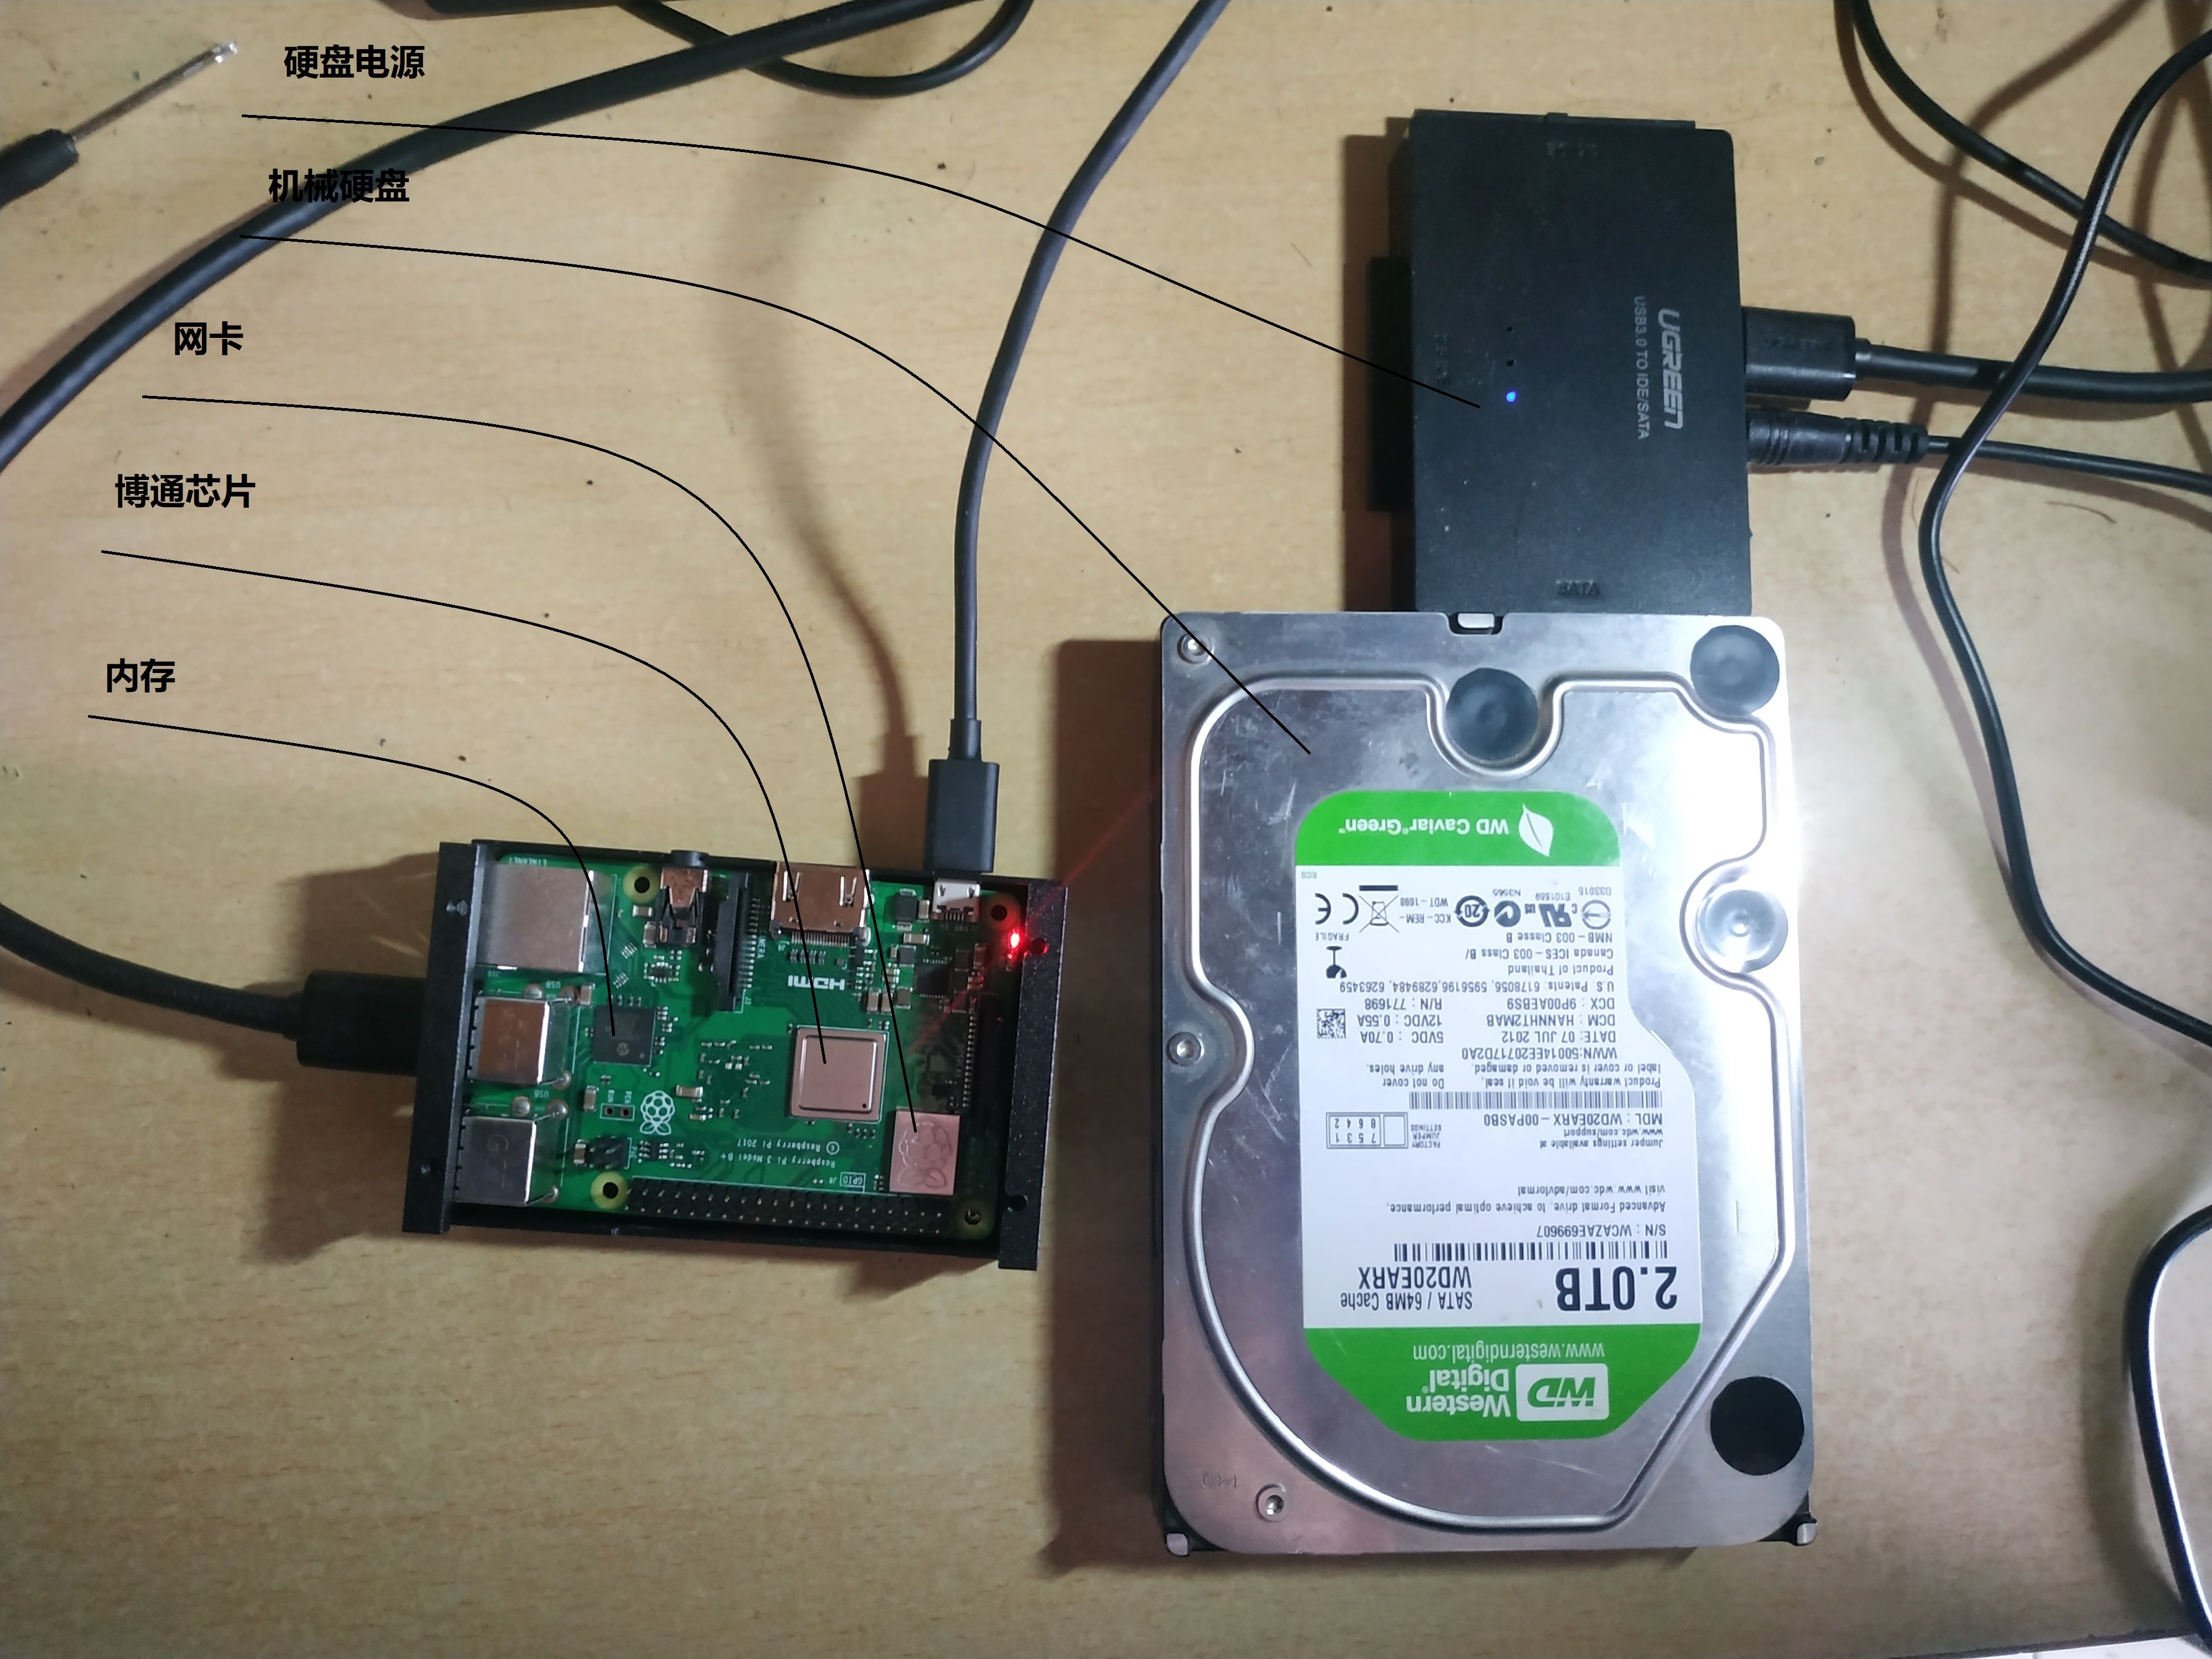
\includegraphics[width=130mm]{./figures/rasberry.jpg}
  \caption{树莓派单片机 2T硬盘}
  \label{raspberrypi}
\end{figure}


\subsection{研究背景}
\paragraph{终端存储空间不足}
对普通的个人消费者用户来说,移动手机还有个人计算机是两种比较常见的终端设备。用户在平时的工作,学习,娱乐中,
会积累下来许许多多的文件,视频,音乐,图片,文本文档,游戏,还有下载的各种资源,这些文件通常占据
了我们绝大部分的存储空间,我们电脑上的存储空间,手机上的存储空间,往往不够用,这时候大家就会想到,将这些文件备
份到云端硬盘中,为本地节省下来存储空间\cite{r7,r9,r10}。

现在市面上主流的手机存储容量一般有16G,32G,64G,128G,256G,然而对于手机用户来说,这些容量往往是不够用的。
现在的手机应用占用的存储空间非常容易能达到300MB以上,QQ微信的空间会更多一点。QQ微信微信照片内容分享,再加上现如今的如今
比较流行的短视频应用,摄像录影对用户来说可以说是绝对的刚需了。这时候一个普通的用户平时的照片视频存下来的话,
没几天消耗的存储空间都能达到上百兆,一张照片有3到5兆的大小,用手机拍摄的没有经过后期的视频一分钟都有150M左右,
很快的手机终端的存储空间被消耗殆尽。当然手机的厂家都会提供自身的云服务,但是在超过免费的存储容量之后,手机厂商
就回收取非常昂贵的云存储费用。

相比使用闪存技术来存储数据的手机来说,个人计算机一般采用128GB,或者256GB的SSD固态硬盘作系统盘,外加500GB,
或者1TB的机械硬盘来做数据存储盘。因此对电脑相对手机来说,存储设备的价格相比手机还是要低一些的,下面是一些固态
和机械硬盘的价格图标,机械硬盘的价格还是可以接受的,但是在终端设备存储数据有一个很大的弊端
就是数据的容灾不能得到保证,因为终端损坏而导致数据丢失用户后悔不及的事情屡屡发生。因此本项目数据和终端的分离就显得
非常有现实意义了。

\begin{figure}[H]
  \centering
  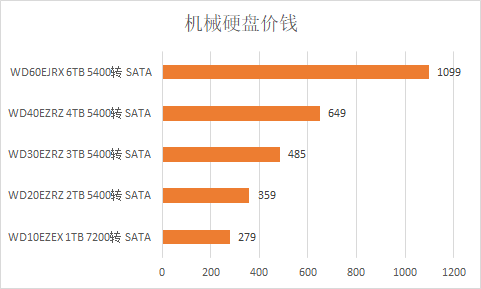
\includegraphics[width=130mm]{./figures/raid2.png}
  \caption{ 西部数据硬盘价钱\cite{r19}}
\end{figure}

\paragraph{云盘服务价格昂贵}
云存储是一项刚需,现在各手机厂商都会有自家的云存储,像苹果的icloud,小米的Mi Cloud等,但是价格并不便宜。
苹果的icloud的一年2TB的存储空间的价格为810元\cite{r22},小米10G就要收费60元,现在市场上比较流行的是百度云,
百度一开始有3TB的免费的存储空间,但是如果你额外要存储更多的数据的话,可以向他购买一年2TB价格为249元
的存储空间套餐,但是百度云对非会员用户来说下载速度有很大的限制,现在百度云将非百度云会员的下载速度限制在500KB/S以下。

国外比较流行的云存储服务,有谷歌的Google Drive,微软的One Drive,亚马逊的Amazon Cloud Driver,
但是国外的云存储服务有两个很明显的缺点,一个是价格,比百度云还要昂贵,而且因为特殊的国情这些国外的云存储厂家都没有
在国内开服务器,在网络的稳定性和速度上有很大的折扣\cite{r11,r12,r13,r14}。相比于各厂商提供的方案,本系统可以提供一种更为经济的云盘解决方案,
就是通过树莓派(英语:Raspberry Pi)和家庭宽带来部署云盘服务。闲鱼上1块2TB的二手机械硬盘,大概需要250块钱左右,
我们知道一块机械硬盘的寿命可以维持在4到5年左右,平均下来每年只需要花90多块钱就可以享受到2TB的存储空间,一个私人的云存储服务,
可以花更少的价钱而得到更大的存储空间。

\begin{figure}[H]
  \centering
  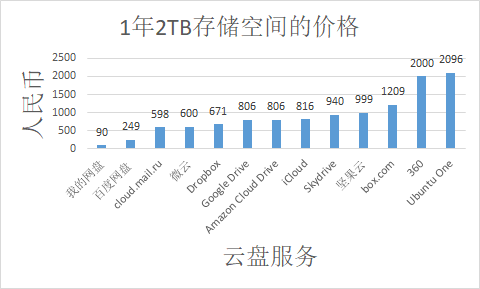
\includegraphics[width=130mm]{./figures/cloud_price.png}
  \caption{市场上主流的云盘服务价钱\cite{r11,r12,r13,r14,r22,r23}}
\end{figure}

当然私人的云盘服务有很大的缺点就是,在文件共享,异地访问,并发访问,相比于成熟的商业公司提供的云存储
服务有很大的缺陷。本项目是利用上海电信提供的20兆家庭宽带,服务器上载速度明显限制在500KB/s以下。在本项目的实验中,
在北京异地访问寝室树莓派上的视频文件只能够保证20KB/s的速度,效果不能令人满意。但是局域网环境下,本系统基本可以做到
1.25MB/s的上载下行速度。

\paragraph{家庭宽带和磁盘资源没有得到充分利用}
家庭宽带和硬盘资源很难得到充分的利用。因为学习和工作的原因,用户不在家时间占了大部分的时间,宽带资源往往得不到充分的利用。
同时因为硬盘技术的发展,旧电脑的机械硬盘被固态硬盘取代,这些淘汰下来的机械硬盘也得不到充分利用。本系统的目的之一就是开发一种
在线存储系统,将这些淘汰的资源充分利用起来。

关于使用旧的硬盘有硬盘损坏数据丢失的风险。机械硬盘的理论寿命大约三万个小时,企业级硬盘、监控用硬盘,如果始终保持高速运转工作,
三年的话就会而损坏,消费者级的硬盘正常使用6到7年是没有问题的,不过硬盘的寿命的的预测大多基于生产数据的结果统计,相关的理论分析还是很缺乏,
也没有相应的研究成果公布\cite{r24}。一般机械硬盘的寿命和它的读写数次数有关,如果频繁读写的话,机械硬盘的寿命会大大的降低,
但是本项目的磁盘独显磁盘读写的场景并不多,而且本项目还做了相对应的增量备份,异地备份,在一定程度上保证了数据安全。

\paragraph{文件增量备份、异地备份}
文件备份的重要性不言而喻,一旦发生灾难或错误操作的时候,我们需要一种手段能够有效的恢复系统的数剧。在文件备份手段方面,
有三个主要的形式,完全备份、增量备份和差异备份,如何在确保数据安全的基础上能够尽量减少存储空间的消耗,这是本系统要解决的难题。
另外,如果要确保数据的容灾,需要做到异地备份,本系统原始数据是存放在家里或者寝室中的机械硬盘中,发生数据损坏的概率很小,
但是数据的重要性是不言而喻的,所以需要做到一点在异地备份的方案中,有两个可选择的方案,一种是成
本比较低的,就是在寝室或者家中各有一个服务器进行备份,另外就是使用亚马逊的aws的s3存储服务,使用云存储的安全性更高,但相应的备份速度
更慢而且成本更高\cite{r25}。有一种方案是二者的结合,在家中和寝室的服务中进行备份的同时,有重要标签的文件使用商业公司提供的云存储服务,这是一个
安全和成本兼顾的方案了。


\subsection{本文贡献}

\subsubsection{云盘系统实现}
\par 本文实现了一个提供文件备份、共享、存储、访问、搜索、管理等功能,满足多终端使用的且部署在单片机树莓派上在线云盘存储系统。
从图\ref{total_system}可以看出树莓派体积非常小,仅有大概4英寸的大小,这意味着
它的能耗非常低。实验数据表明树莓派的平均功耗只有2W/h,意味着如果全年运行树莓派仅仅需要消耗18度电,
但是它的性能完全能够满足文件的上传备份访问、少量并发等基本功能,相比于个人计算机或者是专业的商用计算机来说,
树莓派的功耗可以说是几乎忽略不计\cite{26}。本系统通过路由器的端口映射,提供外网访问的功能,用户可以通过安卓客户端或者
web来访问存储在机械硬盘上的文件。经过测试,局域网内的文件上传能达到19.7Mbps的上载速度,20.4Mbps的下载速度。
本实验的路由器网卡速率为500Mbps,基本上满足局域网的文件访问功能。经过测试,北京访问基于上海电信网络环境
的树莓派上的文件可以达到平均25Kbps的速率,非常遗憾这个速率不能满足异地文件访问的要求。当然网速取决于运营商提供的网络套餐,
没有必要在代码上进行优化,况且本系统的使用场景大多是在寝室局域网和校园网、城域网内,所以像文件的备份和远程访问都是没问题的。
除了性能上的可用性,本系统还实现了Web客户端(图\ref{web_jiemian}、安卓客户端(图\ref{android_jiemian}),用户所需要的基本的云盘
功能都有实现,所以本系统具备功能上的可用性。
\begin{figure}[H]
  \centering
  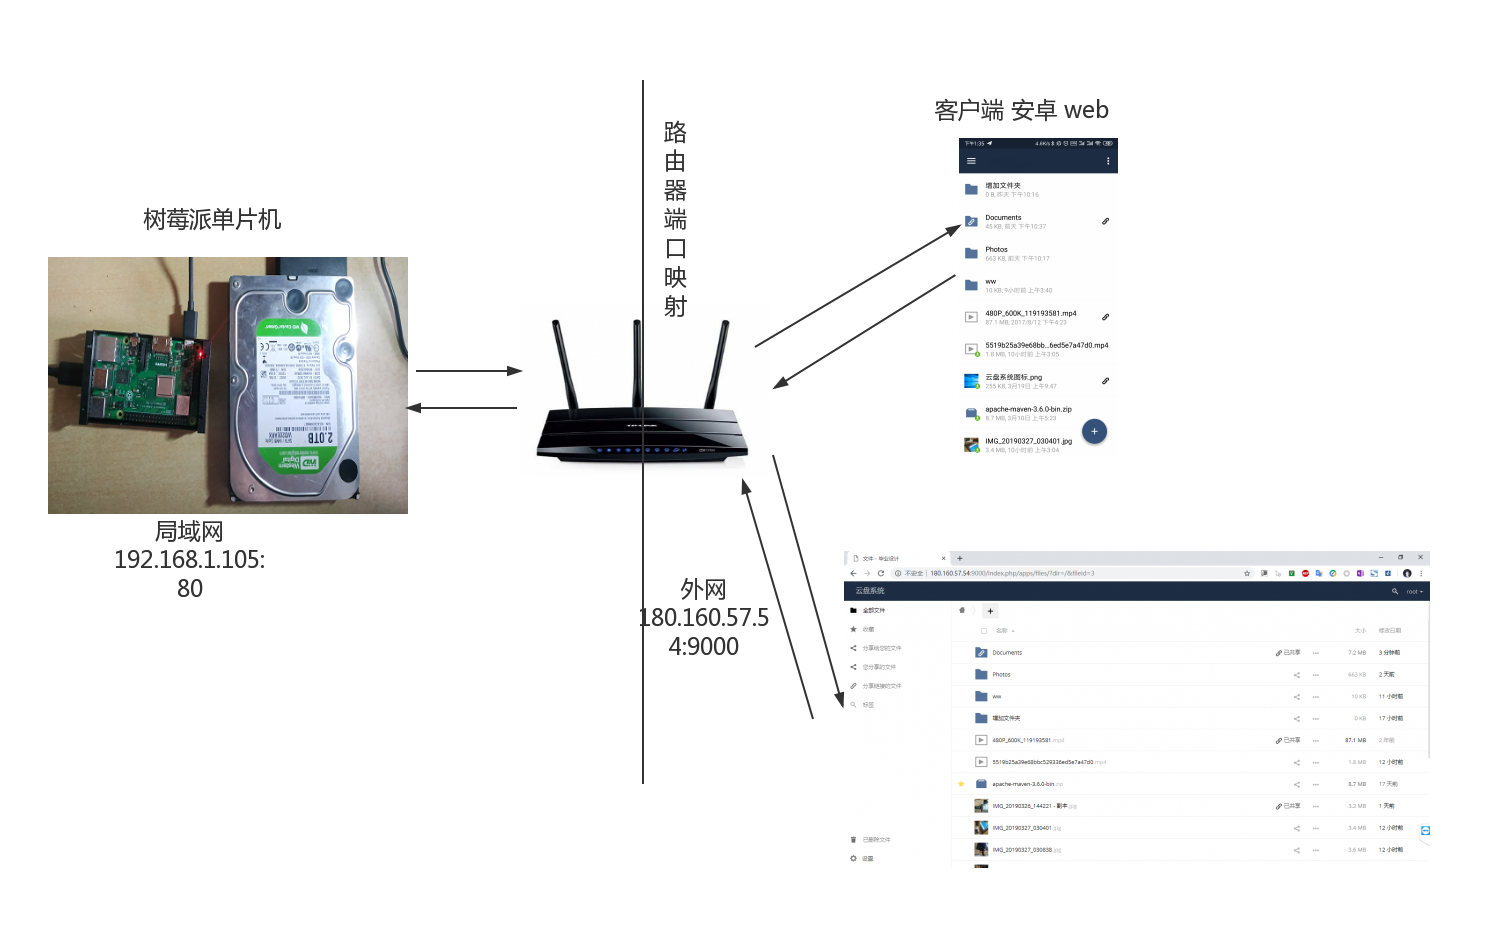
\includegraphics[width=130mm]{./figures/total_system.png}
  \caption{系统总览}
  \label{total_system}
\end{figure}

\subsubsection{Web客户端实现}
\par 本系统Web端基于jquery-ui和bootstrap实现良好的用户界面,用户可以对文件进行增删改查的操作,也可以分享文件,添加标签,
收藏文件,上传下载文件,基于html5视频在线播放,还有图片预览等功能。

\begin{figure}[H]
  \centering
  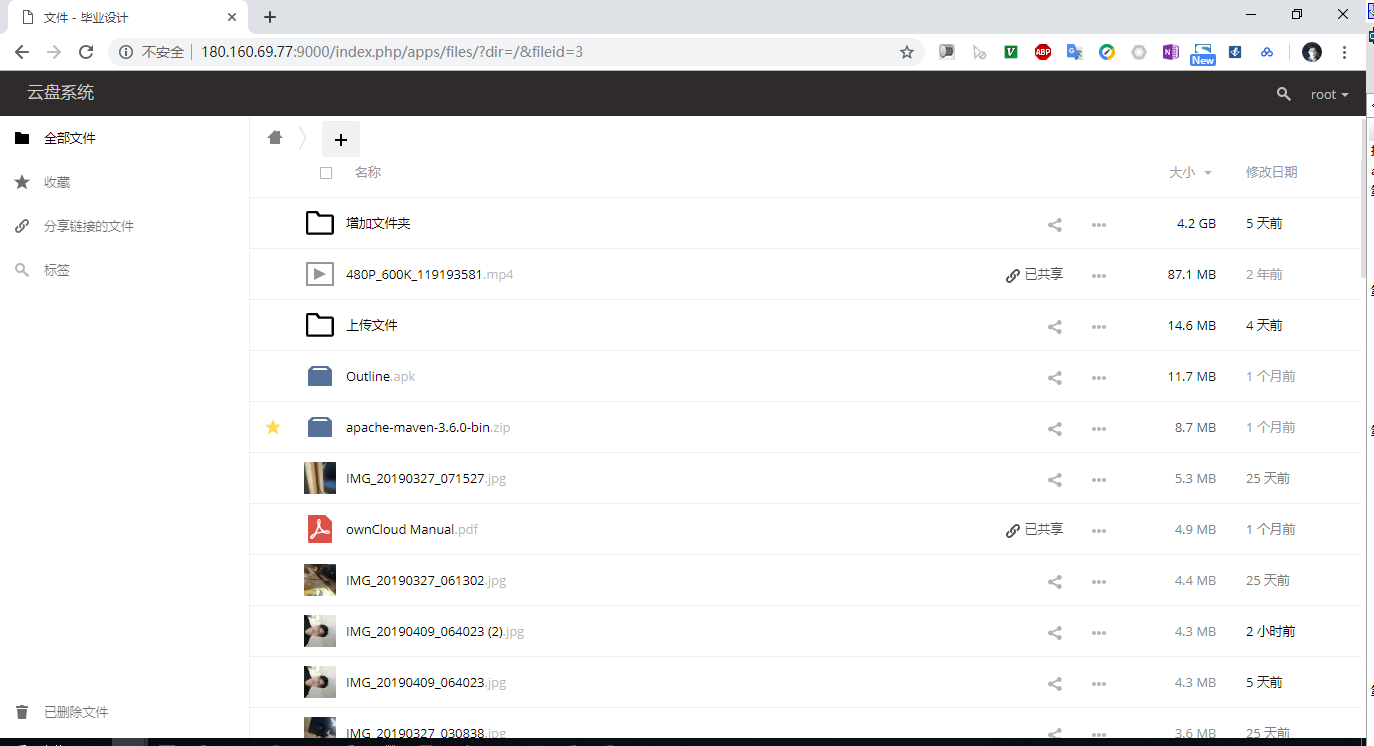
\includegraphics[width=130mm]{./figures/web1.png}
  \caption{web界面}
  \label{web_jiemian}
\end{figure}
\subsubsection{安卓客户端实现}
\par 本系统安卓端基于MaterialDrawer UI框架实现良好的用户界面,基于Volley网络框架实现文件的上传下载,手机图片视频文件
自动上传。
\begin{figure}[H]
  \centering
  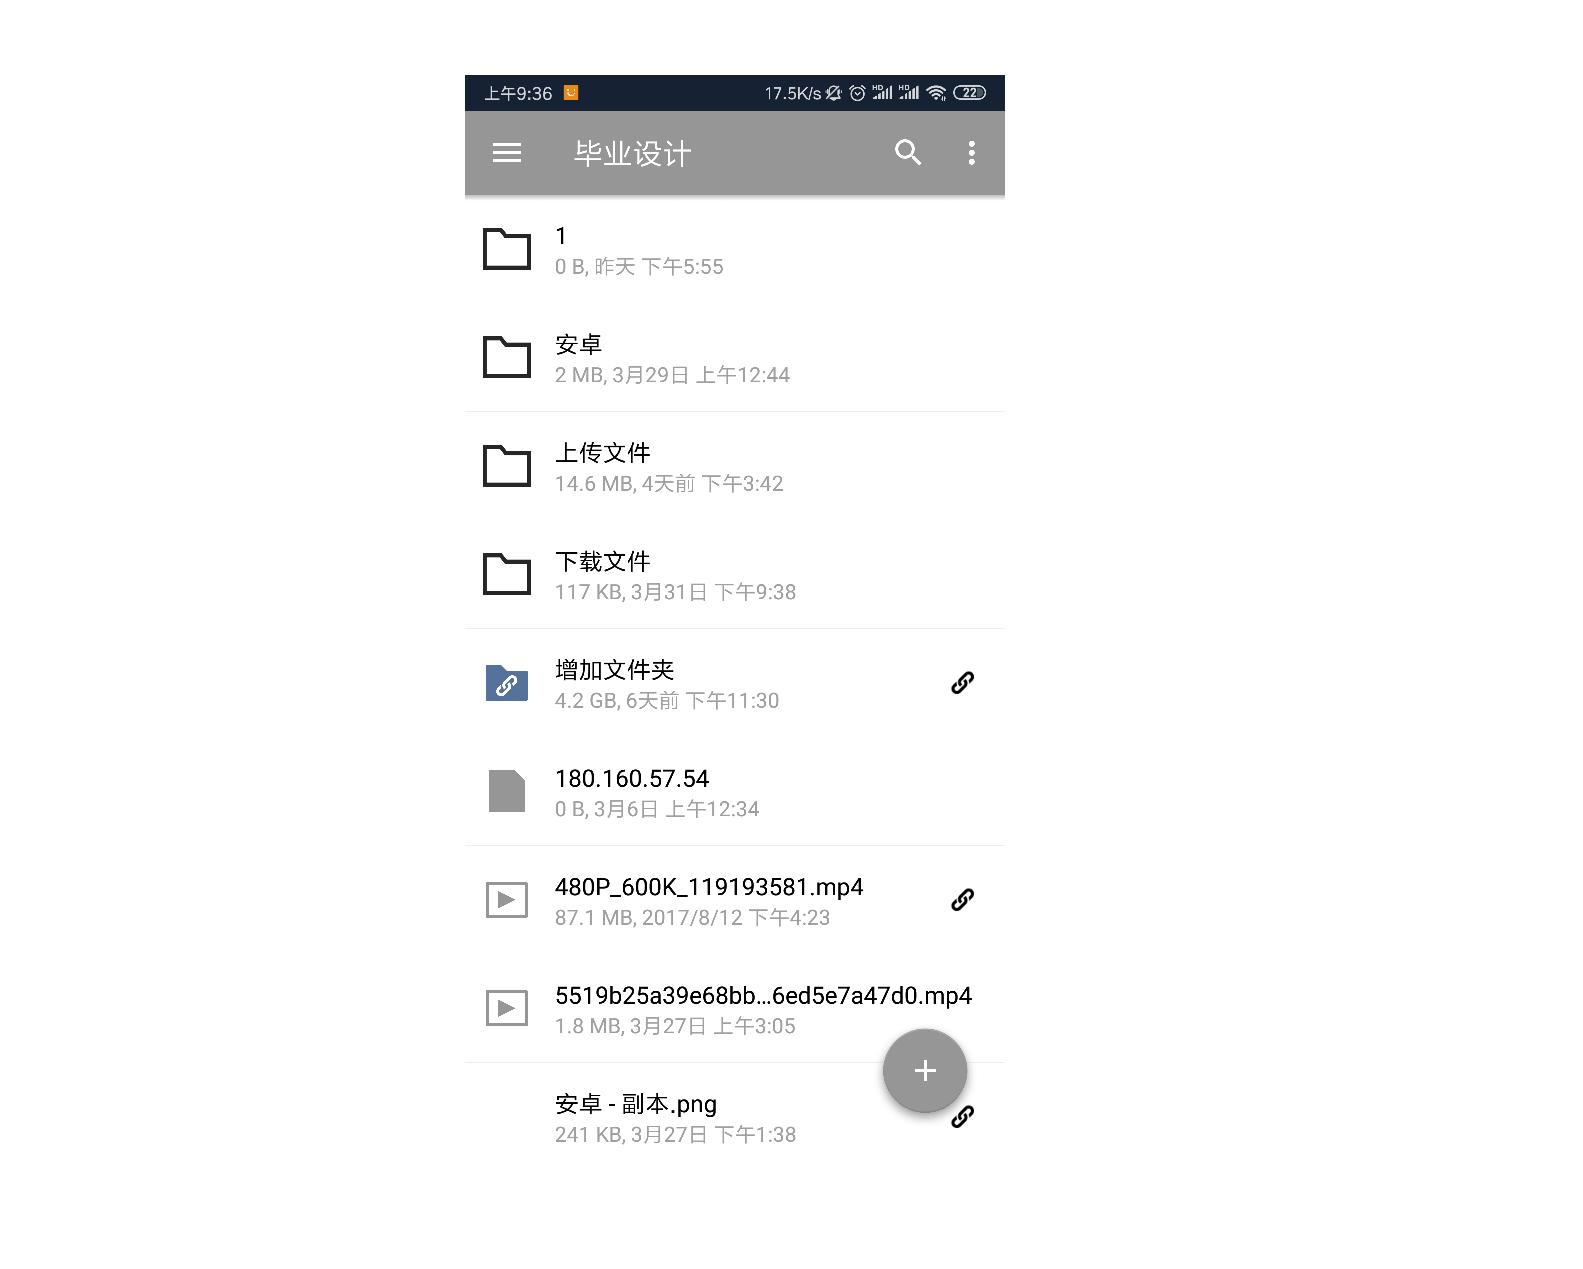
\includegraphics[width=130mm]{./figures/android2.png}
  \caption{安卓界面}
  \label{android_jiemian}
\end{figure}

\subsubsection{安卓端拍摄图片、视频自动上传}
用户可以选在开启或者关闭安卓端的文件自动备份,自动备份的原理是在安卓后台运行一个Service进程对手机/storage/emulated/0下的
目录如图\ref{android_dir}进行监听,当有新文件时会自动读取新文件,通过上传组件与服务器进行交互。因为这一个过程需要大量的后
台资源,手机端的app是默认关闭的。当然为了提升用户体验,也可以设定为在特定时间进行文字备份,比如凌晨时间。
\begin{figure}[H]
  \centering
  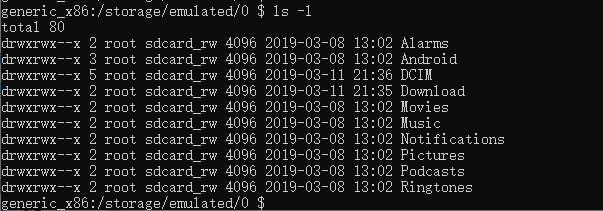
\includegraphics[width=130mm]{./figures/android_dir.png}
  \caption{需要监听的外部存储的目录}
  \label{android_dir}
\end{figure}

\subsubsection{文件增量备份、异地备份}
系统需要至少两台机器来进行文件备份,机器间需要保持数据的同步,如果数据不一致,需要快速的定位到不一致的节点。
本系统实现了在每台机器上针对每个目录数据的散列值维护一棵Merkle树,这样在两台机器间进行数据比对时,从Merkle树
的root节点开始进行比对,如果root节点一样,则表示这两台机器间的目录数据是一致的,不再需要任何处理;如果不一样,
则遍历Merkle树,定位到不一致的节点也非常快速。相比于无脑地对文件进行完全备份,使用文件的哈希值作为文件的身
份标识来构建Merkle树的做法提升了备份的速度和存储空间。

\subsubsection{文件收藏、标签、搜索}
用户可以为文件打上标签,或者收藏,系统会提供额外的分享,收藏,标签,垃圾箱目录给用户访问,用户不用取辛苦寻找标记过的文件。同时系统还提供
文件名模糊搜索(文件限定于在本目录搜索,如果采用和Windows的Exploer的深度全局查找,系统开销会非常大,而且效果不好,一般用户都会记
得特定文件的存放目录,实现文件全局查找实在没有工程上的必要),标签查找。查找结果会动态的在前端页面展示出来,用户体验非常良好。

\subsection{研究思路}
本文从需求分析、概念结构设计、逻辑结构设计、编程实现、实验验证、测试运行几个方面展开研究。
\paragraph{需求分析}
需求分析阶段要对整个云盘系统有一个清晰明确的认识,将各个需求分割成可实现的各个小模块,明确系统的使用场景和面向的使用人群,
指定开发的标准规范,名且系统的设计和实现目标,正对具体业务进行分析和差分,做好业务逻辑说明,明确系统角色,同时要明确哪些
需求是功能性需求,哪些是非功能性需求,这样才能明确重点,提高开发的效率。
\paragraph{概念结构设计、逻辑结构设计}
主要采用E-R模型进行设计,包括画E-R图,然后通过将E-R图转换成表,实现从E-R模型到关系模型的转换,再然后为所设计的数据库选择
合适的存储结构和存取路径。
\paragraph{编程实现}
选定好技术框架后就可以马上动手实现系统了。本系统的技术框架大概有PHP,Apache,MySql,jquery,jquery-ui,bootrap,Android,Volley,
MaterialDrawer UI等。
\paragraph{实验验证、测试运行}
实现主要比较在不通网络环境(局域网,广域网),异地访问,本地访问,WiFi环境,校园网环境、基站流量下对云盘系统的上传下载的速度和
稳定性等基础功能进行测试。功能性测试方面要同时完成网页端和安卓端的单元测试、集成测试、系统测试、性能测试,安全测试、兼容性、接口
测试、极限测试等。性能测试方面要完成对预期性能指标、核心模块并发、组合模块并发、大数据量、疲劳强度、网络性能等多个场景的测试。
并通过实验得到实验数据来完成对系统的可用性和安全性的验证。

\subsection{论文组织}
本文一共分为六个章节,其结构安排如下:

第一章为绪论部分。讲述了本文的研究背景,阐述了本文的研究内容和贡献,并对研究结果做了简单的展示。

第二章为系统需求分析部分。结合文件管理系统实际,分别对系统的总体性需求、功能性需求、非功能性需求、系统技术可行性等几个方面进行介绍和分析。

第三章为系统功能设计部分。在需求分析的基础上对云盘系统进行总体设计,首先介绍了系统设计的目标和原则,在基于以上原则的基础上分别对系统的服务器
架构、使用的一些技术框架,和数据库表格做了详细的介绍和分析。

第四章为系统功能实现部分。在完成功能分析和系统设计之后,此部分详细介绍展示了系统实现的结果,ui界面,系统操作步骤,和一些关键功能的算法实现。

第五章为系统测试与分析部分。此部分结合本系统的实际别对一些常见的测试方法进行粗略的介绍,同时详细介绍了本系统测试时所需要的测试环境和测试工具,
然后本文设计了一些关键的测试用例,并对测试结果进行分析和总结,最后本文用Linux工具dstat对服务器的性能进行粗略的分析。

第六章为总结与展望部分。对本文的主要工作以及创新点进行总结,对未来研究进行展望。                             %
\section{需求分析}
\subsection{系统总体需求分析}
个人计算机和移动手机的存储不足是非常常见的现象,人们迫切地希望能有额外的空间对个人数据进行备份同时还可以方便地访问云端文件。
本系统的目的就是为了解决上诉用户的痛点,同时将闲置的网络和硬盘资源利用起来,起到积极的环保和省钱效果。整个系统具有下面的优点

\paragraph{完善的功能}本系统的个人网盘系统具有文件上传下载、公开分享、用户登录注册、视频在线播放、web端安卓端数据同步、手机文件自动
备份、文件标签、文件搜索、无线添加硬盘存储空间、文件操作符合用户平时在windows、安卓平台习惯的文件操作方式,用户可以没有学习成本就可以
使用本系统,本系统具有以上诸多优点。
\paragraph{先进的文件管理方法}本系统具有明确的管理方法,通过计算机网络技术为用户提供近乎无限的存储空间,解决用户数据丢失的担心,真正做到
方便好用的云盘系统。
\paragraph{成熟的技术}本系统基于主流的系统架构LAMP(Linux、Apache、Mysql、php)来开发,系统具有性能稳定、可扩展性高、安全可用等优点。
\paragraph{操作方便快捷}本系统提供web和安卓两种客户端访问方式,界面美观,操作逻辑符合用户习惯,用户无需特别学习,凭借之前在windows和安卓
平台积累的习惯就可以很快学会使用本系统。经过测试,在局域网的网络环境下,用户上传下载文件,在线视频都可以以接近网卡的速度进行服务器访问,
在广域网的网络环境下,本系统仍然可以提供基本的访问条件。
\paragraph{安全兼容性高}经过测试,本系统的web端在主流的浏览器Chrome、Edge、IE11、QQ浏览器、360安全浏览器、360极速浏览器、百度浏览器、
opera浏览器、手机端的uc浏览器、小米系统浏览器等浏览器都可以正常访问。同时系统的设计具有坚强的安全保密功能对用户个人信息进行保护,并提供
良好的接口,使得文件可以方便的导入导出。

\subsection{功能性需求分析}
在本章节中会介绍本系统所涉及到的功能需求,同时为了方便描述需求,引入了三种用户角色,一种是Web用户、一种是安卓用户、
另一种是非系统用户。非系统用户针对的是所有互联网用户,因为本系统涉及文件的分享,并且提供外网访问本地文件的方式,因此,作为
非本系统用户还是可以访问到系统用户分享后的文件的。

\subsubsection{用户控制需求}
在需求分析开始之初设计了两种注册方式和3种登录方式如下
\par 系统需要支持2种注册方式:
\par 1)账号;
\par 2)手机号,用户输入相应的注册信息完成注册。
\par 系统需要支持3种登录方式:
\par 1)通过账号登录;
\par 2)使用手机号直接登录;
\par 3)通过第三方平台登录,例如微信、QQ等。对于使用手机号登录。

但是在后期的开发过程中,发现注册和登录的功能并不是被系统所关键需要的,因为本系统的定位是局域网内家庭或者寝室成员之间交互,所以完全可以以纯
后端注册的方式来节省开发时间,因此在基于时间紧迫只实现了账号口令登录的功能。

如下用户用例图,web用户和安卓用户都可以进行登录、修改信息等操作,非系统用户不被赋予此项权限。
\begin{figure}[H]
  \centering
  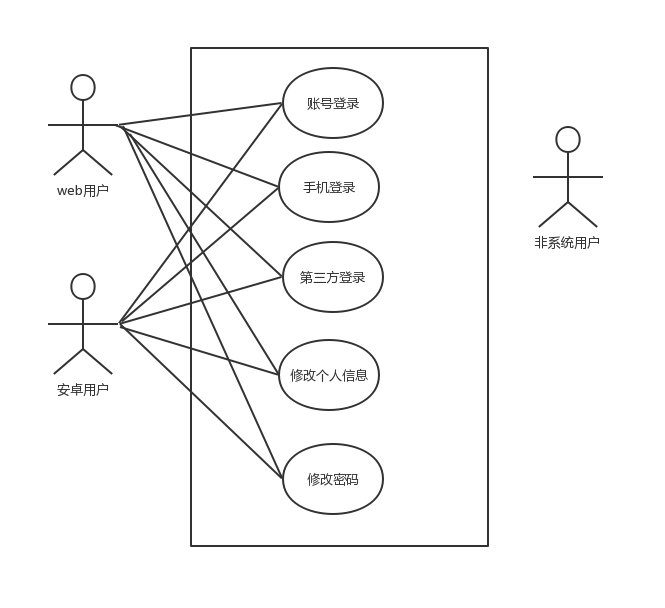
\includegraphics[width=80mm]{./figures/login_yongli.png}
  \caption{用户登录管理用例图}
\end{figure}

\subsubsection{文件/目录操作需求}
本系统提供云存储服务,自然有创建文件/目录、读写文件、删除文件/目录、访问文件/目录属性等。

如下用户用例图,

web用户存在文件上传、文件下载、或许文件详细信息、重命名文件、删除文件、查找文件、分享文件等需求。

安卓用户存在文件上传、文件下载、或许文件详细信息、重命名文件、删除文件、查找文件、分享文件等需求。

非系统用户可以访问下载被分享的文件,但是没有其他操作权限。

\begin{figure}[htbp]
  \centering
  \subfigure[文件管理用例图]{
  \begin{minipage}[t]{0.50\linewidth}
  \centering
  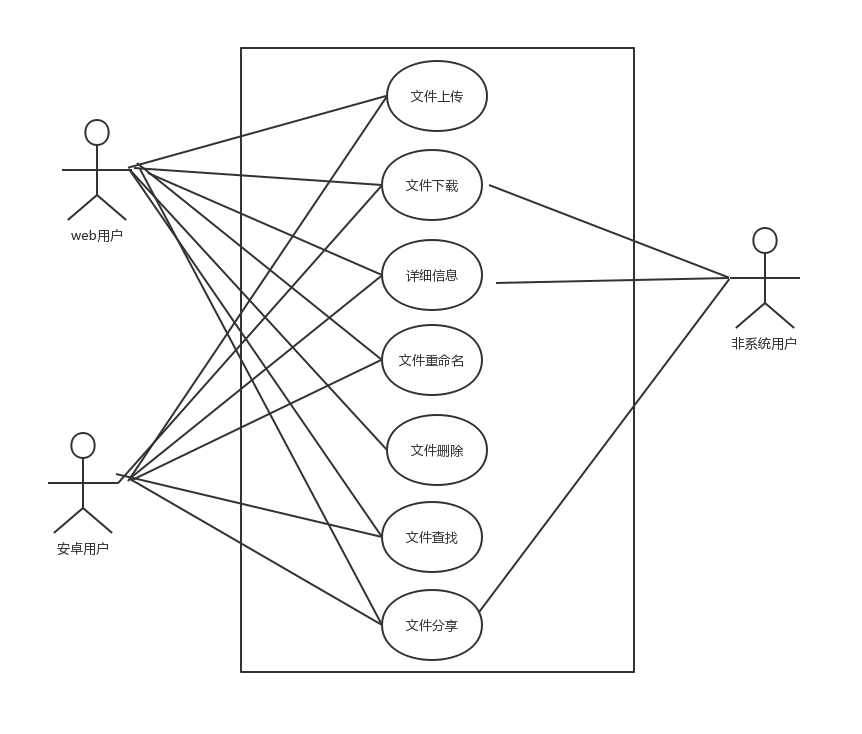
\includegraphics[width=65mm]{./figures/file_admin_yongli.png}
  %\caption{fig1}
  \end{minipage}%
  }%
  \subfigure[文件附加功能用例图]{
  \begin{minipage}[t]{0.50\linewidth}
  \centering
  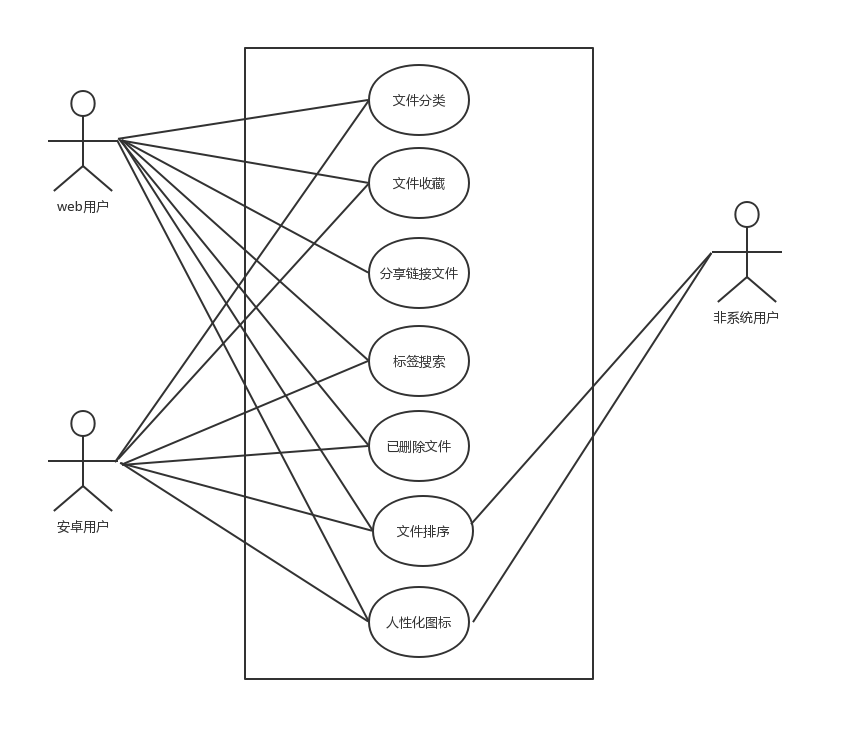
\includegraphics[width=65mm]{./figures/file_attach_yongli.png}
  %\caption{fig2}
  \end{minipage}%
  }%
  \centering
  \caption{文件操作用例图}
  \end{figure}
\subsubsection{文件/目录分享需求}
文件或目录分享是本系统一个非常重要的需求,市场上主流的云盘服务都有提供文件分享功能,同时为了系统安全考虑,
在实现系统的时候需要做一些安全性措施。

如下用户用例图,

web用户存在设置分享链接名称、设置分享密码、设置文件过期时间、修改分享信息、社交分享、访问下载分享文件等需求。

安卓用户存在设置分享链接名称、设置分享密码、设置文件过期时间、修改分享信息、社交分享、访问下载分享文件等需求。

非系统用户可以访问下载被分享的文件,但是没有其他操作权限。
\begin{figure}[H]
  \centering
  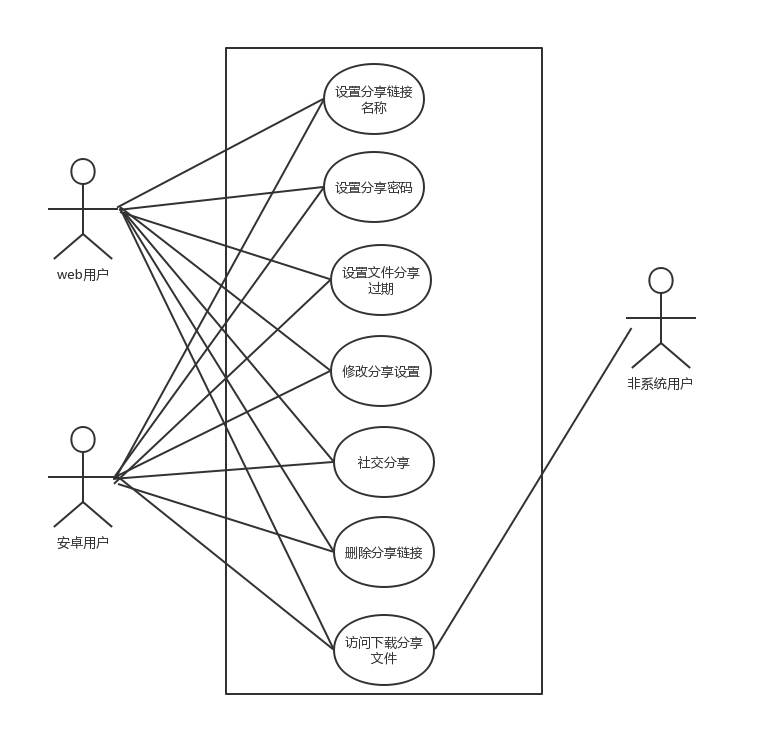
\includegraphics[width=120mm]{./figures/file_share_yongli.png}
  \caption{文件分享用例图}
\end{figure}

\subsubsection{视频在线播放需求}
视频和游戏、社交并称当今互联网三大主流需求,因此在线播放视频是本系统必须要实现的需求了。
本系统采用Apache作为服务器后端,对静态资源的访问有很好的支持,利用html5提供的video元素就可以很方便地实现
流媒体播放的功能,同时Apache对安卓端的VideoView也有很好的支持。

如下用户用例图,

web用户存在视频播放,图片预览、图片视频下载等需求。

安卓用户存在视频播放,图片预览、图片视频下载、图片自动备份、视频自动备份、WiFi环境上传文件、备份后删除原文件节省终端空间等需求。

非系统用户可以访问播放、预览、下载被分享的图片视频文件,但是没有其他操作权限。

\begin{figure}[H]
  \centering
  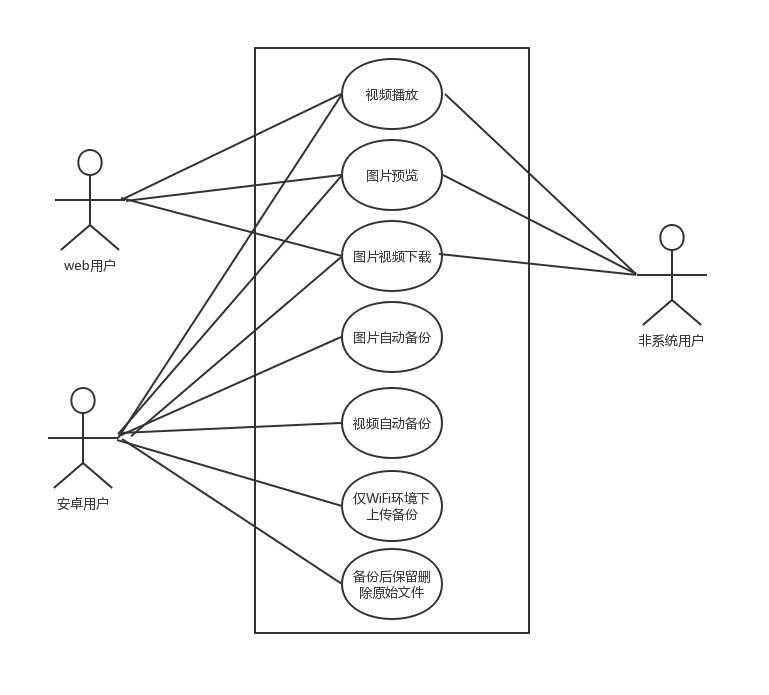
\includegraphics[width=130mm]{./figures/img_video_yongli.png}
  \caption{视频图片文件用例图}
\end{figure}

\subsection{非功能性需求分析}
\paragraph{响应时间} 
响应时间的定义是指一个客户端发送请求到服务器,然后接收服务器响应至结束的这一个过程中总共耗费的时间。响应时间包括三个部分,客户端呈现时间、网络传输时间和服务器响应时间。
其中客户端的呈现时间是指客户端在接收服务器返回的数据后然后渲染成可视化页面所消耗的时间,然后服务器的响应时间是指服务器从接收到客户端发来的请求,然后
在经过一些逻辑操作后(比如查询数据库,业务判断等)向客户端返回数据所消耗的时间。

本系统的使用场景一般位于局域网的环境下,响应时间需要做到基本处于2秒以下。同时如果处于外网的网络条件下,访问带宽也要达到中国电信所给予的500KB/S上载速度,
响应时间也需要做到5S以内。同时本系统是云盘系统,提供文件上传下载功能,因此网络的稳定性和速度都是重要的考量。其实就树莓派和路由器来说,网卡速度最大500Mb/s,因此
在软件算法上提升速度没有太大的意义,后期测试过程中,大文件的上传下载速度基本能保持在1.25MB/s左右的速度。

\paragraph{并发用户数}
并发的定义是多个用户在统一的时间点发送同一件事情或者操作的请求,这些操作一般都是相同的事务行为。
比如用户在互联网抢票的时候,会频繁的刷新结果,导致服务器不堪重负。再比如在文件上传的业务中,不同的用户可能上传相同名称的文件
并且在同一路径下,这时候就需要对该文件加锁才能保证后来的文件不会覆盖已有的文件了。同时,多个用户同时上传文件对孱弱的家庭宽带来说是
不小的挑战,因此并发量达到3个并发用户就可以满足本系统一开始的设定了。
  
\paragraph{吞吐量}
吞吐量的定义是指单位时间内系统接收并处理用户发起请求的数量,同时能够非常直观地体现服务器系统的性能承载力。
对于具有交互式性质的应用系统来说,吞吐量可以体现服务器系统所承受的性能压力。
在各种测试场景中,吞吐量一直都是一个重要指标,它可以在database、middleware和计算机硬件上得到直观的体现。
系统性能瓶颈可以用吞吐量来协助分析,还可以在设计软件性能测试场景用到吞吐量指标来衡量软件性能是否达到了预计的设计目标,
比如交互式应用系统中的Connection Pool、数据库事务发生频率、次数等。

\paragraph{资源利用率}
资源利用率是指对对计算机系统硬件和网络资源的利用程度,例如服务器的CPU利用率、内存利用率、磁盘利用率、网络利用率、GPU利用率等。
同时在改善系统性能的时候可以用资源利用率作为分析判断的重要指标。

在本系统的性能需求章,需要满足下列的性能指标。
\par(1)CPU使用率上限不超过百分之八十五
\par(2)内存利用率上限不超过百分之八十五
\par(3)磁盘I/O交换率上限不超过百分之八十五
\par(4)网络带宽平均可保持在1.25MB/s以上

\subsection{系统可行性分析}

\subsubsection{操作可行性分析}本系统的操作界面力求简洁明了,简化操作流程,使操作尽量符合用户的使用习惯和文件管理规范,用户无需特别学习就简单
上手,因此本系统的操作可行性是绝对可以的。
\subsubsection{技术可行性分型}
LAMP(Linux、Apache、MySQL、PHP)技术架构在世界范围内有非常广泛的应用,根据统计数据,世界上大约百分之七十2的网站都是基于LAMP
技术框架搭建。LAMP由Linux系统,Apache容器,Mysql数据库,PHP、Python等动态语言组成一个非常轻量和灵活的技术框架,开发环境的搭建也非常
方便,在github上有一键安装LAMP的脚本项目,受到世界上不少开发者的欢迎\cite{r27}。同时因为这个技术框架中所有组成产品均是开源软件,很多互联网企业的商业
应用都是采取这个架构,在开发成本和速度上有着明显的优势。J2EE也是开源产品,但是J2EE架构源、轻量、快速开发这些方面和LAMP相比处于劣势。
微软的 dot NET架构在通用、跨平台、性能、价格等方面也是明显不如LAMP架构,因此LAMP无论是性能、质量还是价格都是开发本云盘系统的第一选择\cite{r28,r29}。

本系统LAMP(Linux,Apache,Mysql,PHP)架构模式中,Linux基于Debian版本,具有稳定性强,升级方便,软件包丰富,性能优越,开发简单
等优点。同时采用Apache作为服务器,是因为Apache对静态资源的访问非常友好,避免了开发对静态资源的手动处理,大大节省了开发时间。
服务器规定了统一的API接口,无论是web客户端,还是手机APP客户端都可以采用统一的接口访问到服务器的资源,大大提升了开发效率。
同时数据库采用了开源的Mysql数据库,树莓派上Mysql版本是mariadb,相比于Oracle,MySQL具有开源免费,轻量易用,开发方便的优点,是互联网最流行的数据解决方案。
在本云盘系统中,所有用户信息、文件路径信息、分享文件信息、系统配置信息和其他类型的信息都存储于数据库中,通过SQL语言可以很容易地查询这些信息。PHP是开源的动态语言,它既可以用来做后台业务逻辑的开发,
也可以嵌入到HTML中实现前端效果,也可以访问MySQL数据库中的数据和 Linux 提供的一些特性的动态内容。因此PHP非常适合web开发和为Android数据访问提供接口。
同时因为服务器是部署在中国电信给予的局域网内,所以如果需要外网访问,就需要进行端口映射,端口映射的时候要避免将外网端口设置成常见的80端口,
因为中国电信会为了网路安全,对特定端口不允与开放。同时系统后台会开放一个备份进程,定时对文件进行备份。
\newpage
                             %
\section{系统设计}
\subsection{系统设计目标和原则}
本系统旨在设计和开发一个适合少量并发,大部分局域网场景下,提供文件的上传、下载、分享、搜索、备份、视频播放等功能,
并且使这些功能在实现后易于上手使用,运行稳定并且具有良好的用户经验和可靠的安全性。 因此在设计系统中过程中必须遵循以下原则:
\par 符合开发规范:遵循系统开发各项相关标准和体系。
\par 选用成熟技术方案:为了保证开发效率和开发质量,成熟的技术方案可以保证系统的稳定性和低学习成本,因为网上的资料会比较多。
\par 完善的功能:在需求分析阶段提出的功能尽量完成,为用户提供可行的解决方案。
\par 可扩展性强:系统开发时长期的过程,需求也是不断发生变化,因此设计的时候尽量采用设计模式,预留接口,二次开发才能高效进行。
\par 维护简单:系统需要长期稳定运行,而长期稳定的运行离不开日常的维护。
\par 界面简洁,功能易用。

\subsection{服务器设计}
本云盘系统的服务器设计采用经典的LAMP架构,处理一次客户端动态资源请求的过程如图\ref{lamp_server}
所示,
\paragraph{服务器处理流程} $\mathbb{}$ $\mathbb{}$
\par a) Client发起http请求
\par b) Httpd Server Apache接收请求并交给CGI进程处理
\par c) 通过CGI接口访问PHP的的应用程序
\par d) PHP应用程序调用PHP解释器执行PHP代码
\par e) PHP程序通过Mysql驱动访问数据库数据
\par f) PHP对数据进行封装,最后给客户返回相应
\par 故在LAMP的环境机构中,apache、mariadb和php的主要功能分别如下。

\paragraph{apache主要实现如下功能:} $\mathbb{}$ $\mathbb{}$
\par a) 处理http的请求、构建响应报文等自身服务;
\par b) 配置让Apache支持PHP程序的响应,修改apache conf目录下的httpd.conf配置文件,引入PHP模块;
\par c) 配置Apache具体处理php程序的方法,在本系统中统一使用路由表来出来方法和路径映射;
\paragraph{mariadb主要实现如下功能:} $\mathbb{}$ $\mathbb{}$
\par a) 提供PHP程序对Mysql数据库数据的写入;
\par b) 提供PHP程序对Mysql数据库数据的读取;
\par c) 通常情况下从性能的角度考虑,尽量实现数据库的读写分离,但是本系统地位是个人的云盘系统,因此并发场景不多,所以没有实现读写分离
\begin{figure}[H]
    \centering
    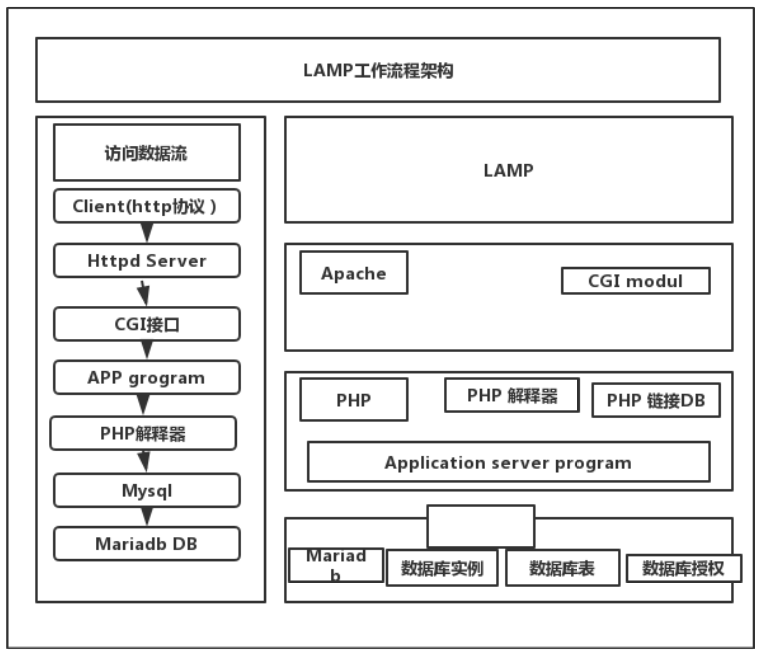
\includegraphics[width=130mm]{./figures/lamp4.png}
    \caption{LAMP架构图}
    \label{lamp_server}
\end{figure}
\paragraph{php主要实现如下功能:} $\mathbb{}$ $\mathbb{}$
\par a) 实现Apache的访问接口CGI,一般用户请求都交给CGI处理,相当于Tomcat中的servlet方法。对于Apache对静态资源的访问可以不经过CGI接口;
\par b) 提供PHP程序的解释器;
\par c) 提供Mysql数据库的访问驱动,驱动是为了将数据库的磁盘比特转化成PHP可以识别的数据结构。

具体的服务器设计如图\ref{server_img}所示。经过路由器端口映射,客户端可以在外网或者局域网的网络环境下访问服务器,在服务端,系统实现了动静资源的分离,如果是直接访问文件,直接经过
apache的路径就可以不需要php来处理请求了,直接返回静态文件资源。同时系统会添加新进程,进行文件的增量备份和异地备份。

\begin{figure}[H]
    \centering
    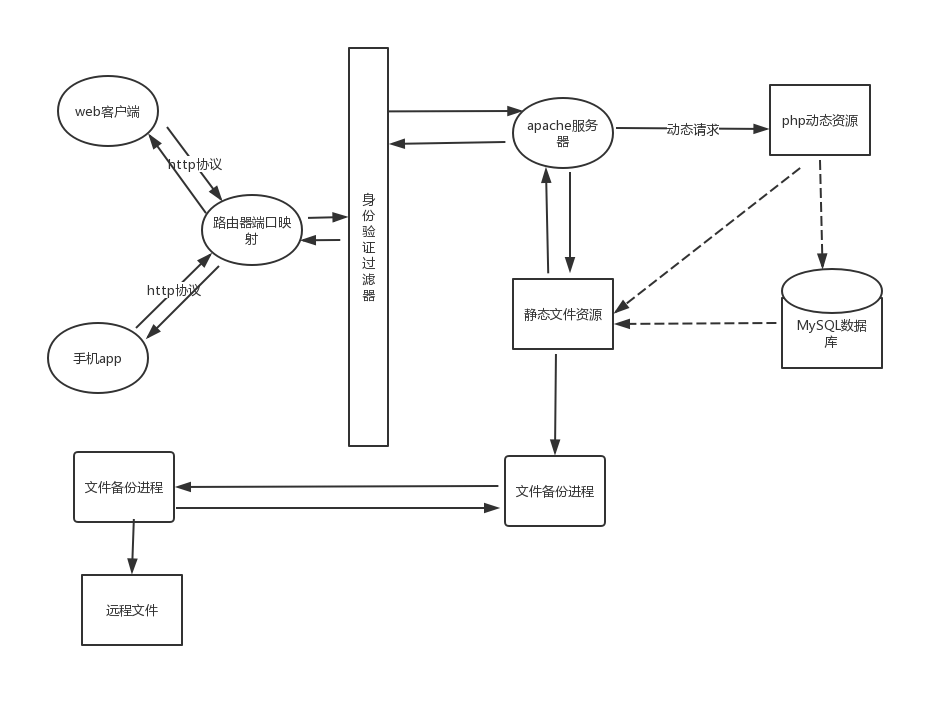
\includegraphics[width=130mm]{./figures/server.png}
    \label{server_img}
    \caption{系统总架构图}
  \end{figure}

\subsection{数据库设计}
根据系统的各个功能模块的划分和各个系统角色的从属关系,设计了一下的数据库系统,第一部分是从全局的视角展示各个系统角色之间的关系,
接下来再详细地介绍各个表字段的含义。

本文的系统数据库表格设计主要分为3个模块,分为用户模块、文件模块、系统配置模块。用户模块和文件模块有依赖关系,
系统配置模块需要规定服务器系统的硬件配置、允许访问的外网ip、内网ip、文件根路径、存储空间大小等信息。用户模块包括OcAccount、
OcMounts、OcUsers 3张表,文件模块包括OcMinetypes、OcShare、OcFilecache、OcFileTrash、OcSystemtagObjectMapping、OcSystemtag 6张表,
配置模块包括OcAppconfig、OcAppconfigKey、OcAuthtoken、OcAuthtokenWithBLOBS 4张表。

在概念设计的基础上,可以在数据库中完成实际的建表,同时建立各个表互
相之间的外键联系。在数据库的设计过程中,需要遵循一定的设计规范,以减小
数据的冗余,提高数据访问效率。本系统选用MySql 5.7版本的数据库进行
开发,需要建立的表包含系统用户、文件类型、分享文件、垃圾文件、基本文件、
文件标签、标签文件关系映射。遵循统一化驼峰法命名原则,每个表的命
名都以Oc(Own Cloud)开头,最后部分为表名称的英文。云盘系统的核心
功能的表物理结构如表\ref{user_table} \ref{type_table} \ref{share_table} 
\ref{trash_table} \ref{file_table} \ref{tag_table} \ref{middle_table}所示。

\begin{figure}[H]
    \centering
    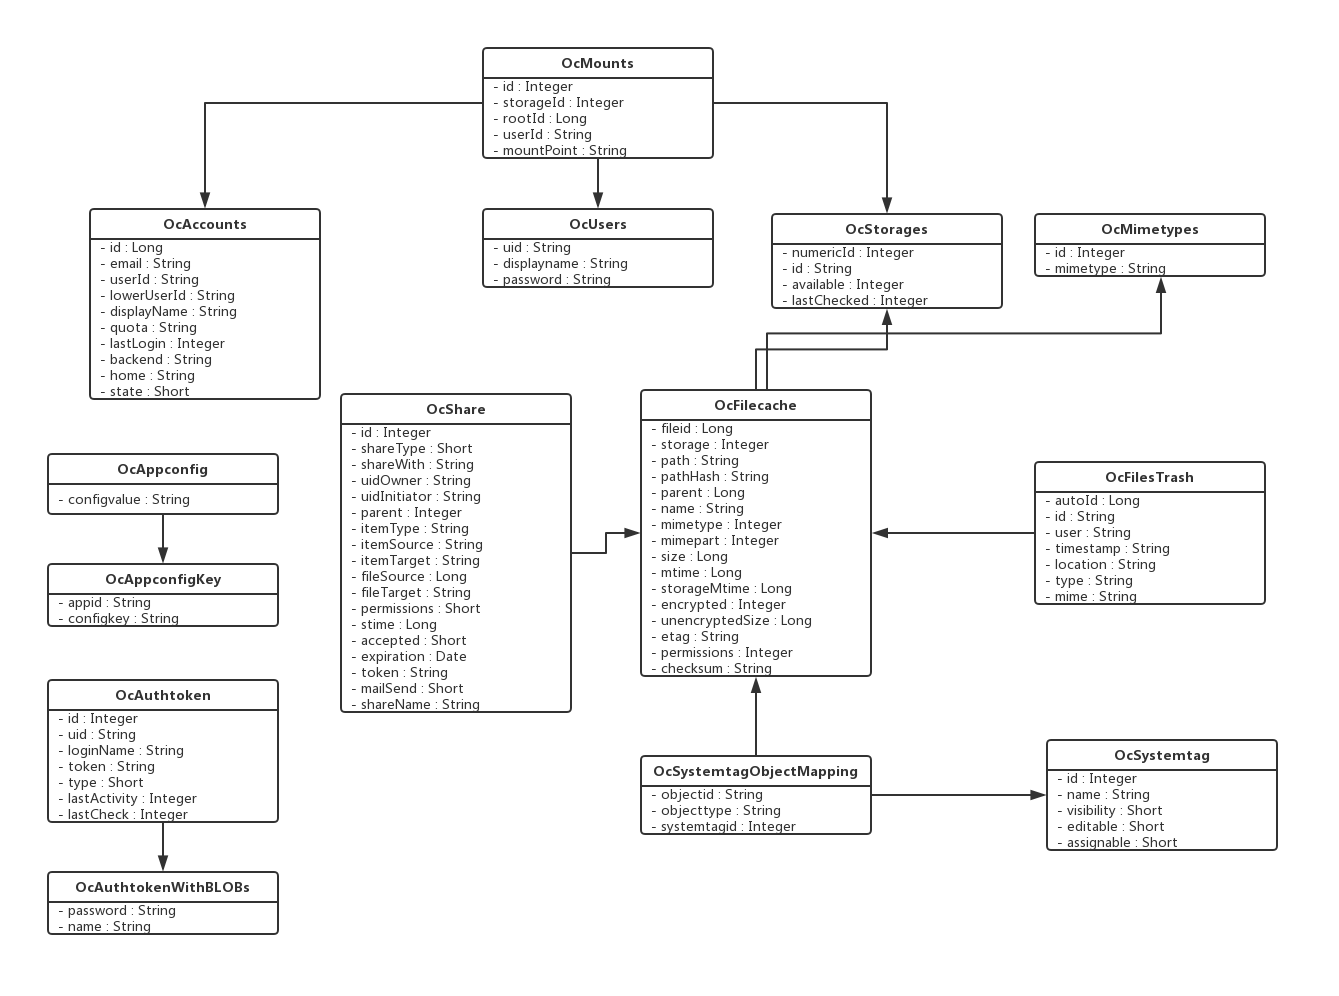
\includegraphics[width=130mm]{./figures/classes.png}
    \caption{数据库总类图}
  \end{figure}

\paragraph{用户基本信息表}
用户基本信息:包括用户id、用户昵称、口令、邮箱、存储外键、上次登录时间、家目录、用户状态。

\begin{table}[htbp]\center
    \caption{OcUsers 用户表}
    \begin{tabular}{lcccccl}
     \toprule
     字段名 & 数据类型 & 说明 \\
     \midrule
     uid         & String  &  用户id        \\
    displayname  & String  &  用户昵称      \\
    password     & String  &  口令(哈希过)\\      
    email        & String  &  邮箱          \\
    storageId    & Integer &  存储外键      \\
    lastLogin    & Integer &  上次登录时间  \\
    home         & StringA &  家目录       \\
    state        & Short   &  用户状态      \\
     \bottomrule
    \end{tabular}
    \label{user_table}    
   \end{table}

\paragraph{文件类型基本信息表}
文件类型基本信息:文件存在视频、图片、文件夹、二进制文件、可编辑文本文件、音频文件等类型
\begin{table}[htbp]\center
\caption{OcMinetypes 文件类型表}
\begin{tabular}{lcccccl}
    \toprule
    字段名 & 数据类型 & 说明 \\
    \midrule
    id         & Integer  &  id        \\
    mimetype  & String  &  文件类型      \\

    \bottomrule
\end{tabular}
\label{type_table}   
\end{table}

\paragraph{分享文件基本信息表}
分享文件基本信息:id、用户id、分享文件是文件夹类型还是文件类型、文件路径、是否允许共享、分享时间、文件身份标识、分享文件名、分享链接过期时间等

\begin{table}[htbp]\center
\caption{OcShare 分享文件表}
\begin{tabular}{lcccccl}
    \toprule
    字段名 & 数据类型 & 说明 \\
    \midrule
    id          & Integer  &   id      \\
    uid         & String   &   用户id   \\
    itemType    & String   &   文件夹或文件    \\  
    fileTarget  & String   &   文件路径     \\
    permissions & Short    &   是否允许共享\\
    stime       & Long     &   分享时间  \\
    token       & String   &   文件身份 \\     
    shareName   & String   &   分享名字  \\    
    expiration  & Date     &   过期时间   \\
    \bottomrule 
\end{tabular}
\label{share_table}   
\end{table}

\paragraph{垃圾文件信息表}
垃圾文件信息:包括id、用户id、时间戳、位置等信息。用户可把不用的文件放入垃圾箱,系统默认保存1个月的时间,在一个月时间内,用户可恢复文件,否则系统会在物理存储设备中删除文件。

\begin{table}[htbp]\center
\caption{OcFilesTrash 垃圾文件表}
\begin{tabular}{lcccccl}
    \toprule
    字段名& 数据类型 & 说明 \\
    \midrule
    id         &    String    & id   \\
    user       &    String    & 用户   \\
    timestamp  &    String    & 时间戳   \\
    location   &    String    & 位置   \\
    \bottomrule 
\end{tabular}
\label{trash_table}   
\end{table}

\paragraph{基本文件信息表}
基本文件信息: 这个表是系统的基本文件表,对文件的增删改查就是基于此表。主要包括文件id,存储,路径,路径哈希,父目录,文件名,文件类型,文件大小,上传时间,源文件创建时间,是否压缩,压缩后文件大小,文件标签,文件哈希值等信息。

\begin{table}[htbp]\center
\caption{OcFilecache 文件表}
\begin{tabular}{lcccccl}
    \toprule
    字段名& 数据类型 & 说明 \\
    \midrule
    fileid         & Long  &  文件id \\
    storage        & Integer  &  存储 \\
    path           & String  &   路径\\
    pathHash       & String  &   路径哈希\\
    parent         & Long  &   父目录\\
    name           & String  &   文件名\\
    mimetype       & Integer  &  文件类型\\
    size           & Long  &  文件大小 \\
    mtime          & Long  &  上传时间 \\
    storageMtime   & Long  &  源文件创建时间 \\
    encrypted      & Integer  &  是否压缩 \\
    unencryptedSize& Long  &   压缩后文件大小\\
    etag           & String  &  文件标签 \\
    checksum       & String  &  文件哈希值 \\
    \bottomrule 
\end{tabular}
\label{file_table}   
\end{table}

\paragraph{标签表信息表}
标签表信息:用户可以为每个文件打上标签,方便日后查找,同时用户可以为单个文件打上多个标签。主要有标签id,标签名,是否可见,是否可编辑等。

\begin{table}[htbp]\center
\caption{OcSystemtag 标签表}
\begin{tabular}{lcccccl}
    \toprule
    字段名& 数据类型 & 说明 \\
    \midrule
id          & Integer & 标签id\\
name        & String  & 标签名\\
visibility  & Short   & 是否可见\\
editable    & Short   & 是否可编辑\\
    \bottomrule 
\end{tabular}
\label{tag_table}   
\end{table}

\paragraph{标签文件中间表}
因为标签和文件之间是多对多的关系,所以需要一个中间表完成对二者关系的映射。标签文件中间表基本信息:文件id、标签id
\begin{table}[htbp]\center
\caption{OcSystemtagObjectMapping 标签文件中间表}
\begin{tabular}{lcccccl}
    \toprule
    字段名& 数据类型 & 说明 \\
    \midrule
    objectid    &  String  & 文件id\\
    systemtagid &  Integer  & 标签id\\
    \bottomrule 
\end{tabular}
\label{middle_table}   
\end{table}
\newpage                             %
\section{系统实现}
\subsection{系统实现环境}
树莓派、2T西部数据机械硬盘、机械硬盘电源、500Mb/s网卡速率TP-Link路由器
\subsection{系统功能实现}

\subsubsection{用户登录}
登录注册需要一个很长的验证过程,下面的流程图给出很了很详细的验证过程。登录注册的流程图是功能需求分析的时候开始设计,考虑了很多因素进去,
包括了更重成功、失败结果如何进行处理。但是因为开发时间紧迫,目前本系统只实现了用户名,口令登录部分,剩下的部分在之后的完善计划中会有进一步
的工作。

因为本系统Web端和安卓转都使用同一的接口进行登录,所以服务器会返回一个同一的requesttoken作为身份验证。传统的浏览器登录方案中,是浏览器发送的
登录请求在服务器验证通过之后,服务器发回SESSIONID和重定向地址,浏览器会自动将SESSIONID地存入Cookie中作为下次请求的身份验证。服务器端会
使用基于动态代理实现的面向切面编程的思想对所有请求进行拦截做身份验证,一般服务器会在SESSION中存有登录成功后的用户信息,服务器端的SESSION
相当于一张hash表,根据客户端请求头中cookie值来判断SESSION中是否保存有用户信息,如果没有,那么就说明发送请求的客户端处于非登录状态,
那么服务器就会发回402代码,如果存在用户信息,那么就会将客户端请求放行。

\begin{figure}[H]
  \centering
  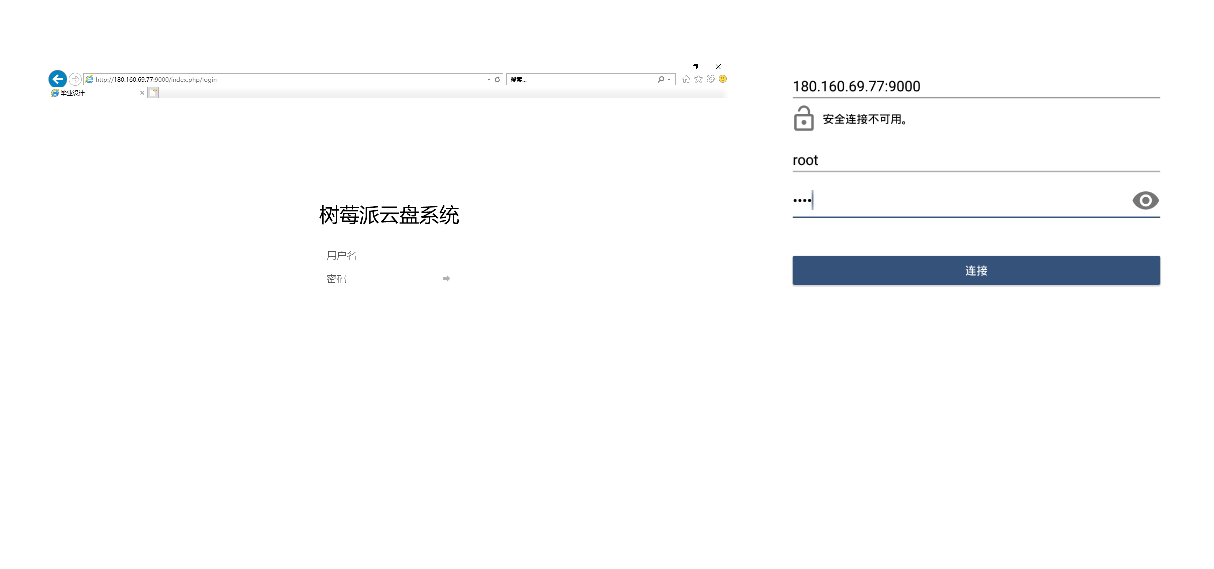
\includegraphics[width=130mm]{./figures/android_web_login.png}
  \caption{安卓、网页登录界面}
\end{figure}

不同于传统的登录实现方案,本系统存在安卓客户端和web客户端,为了避免写两套接口实现一样的功能从而带来开发效率的降低,服务器采用restful的
思想统一web客户端和安卓客户端的接口。所以本系统的登录验证过程是这样的,客户端发送登录初始请求,服务端生成requesttoken并保存在SESSION中,
并返回requesttoken,在web端,浏览器会把requesttoken写入Cookie中。安卓端的网络层使用Retrofit2 + RxJava + Okhttp3框架,安卓端在接收到
requesttoken后,会对requesttoken进行持久化处理,然后当每次使用Retrofit发送请求时,就会在Retrofit请求头中加入requettoken的头部信息,从而
达到身份验证的效果。
\begin{figure}[H]
  \centering
  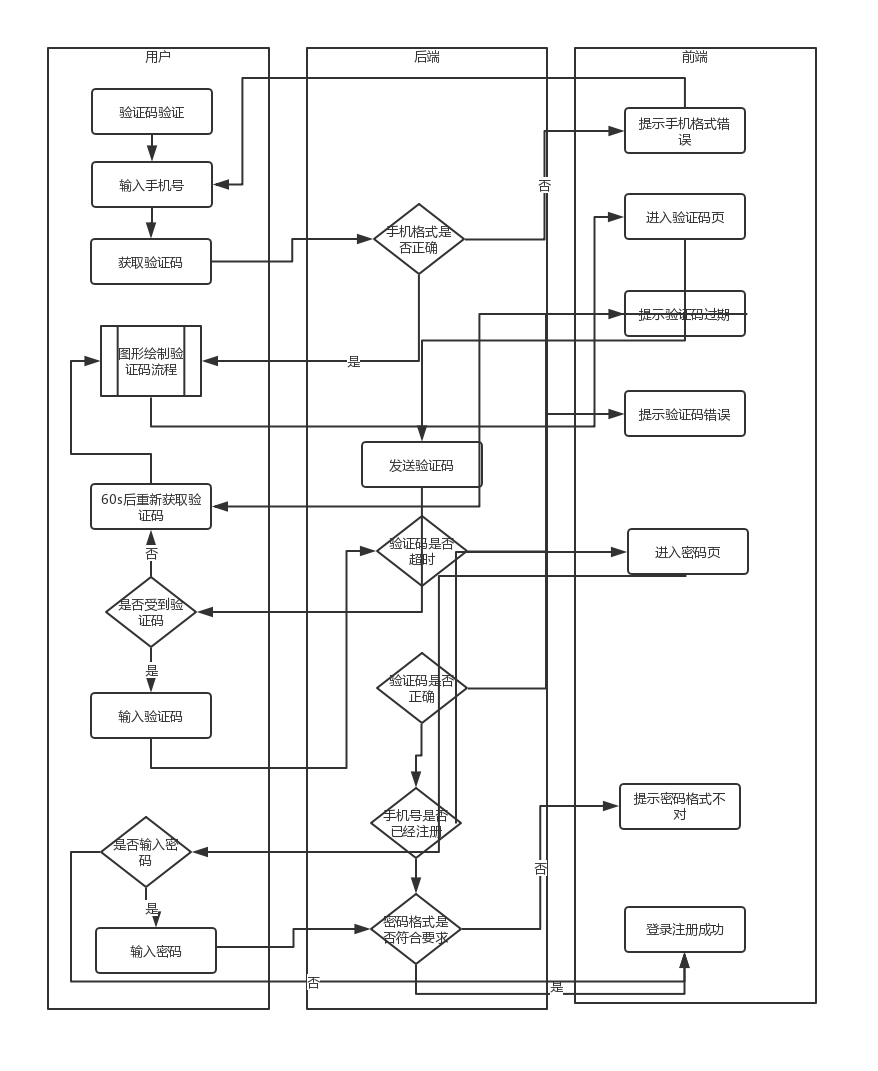
\includegraphics[width=130mm]{./figures/login_liucheng.png}
  \caption{登录注册流程}
\end{figure}

\subsubsection{文件上传}
要保证大文件上传下载的完整性,就需要断点续传的解决方案。

基本的思路是基于阻塞队列BlockingQueue使用生产者消费者模式,
开启读文件线程将大文件切割成固定大小的part,读取后存入阻塞队列BlockinQueue中,
同时开启上传线程将BlockingQueue中part上传。
BlockinQueue为固定大小,在本系统中设置为cpu的核心数4,如果BlockingQueue中
的part数量大于BlockingQueue容量,则读文件线程陷入阻塞状态,如果BlockingQueue为空,
则上传进程陷入阻塞状态,同时,如果读文件读完文件,会将NULL值加入BlockingQueue中,
当上传线程读到NULL时,代表所有文件块已经全部上传,这时会通知服务器对文件进行合并\cite{r30}。

下面给出了本系统使用多线程断点下载的流程图。
\begin{figure}[H]
  \centering
  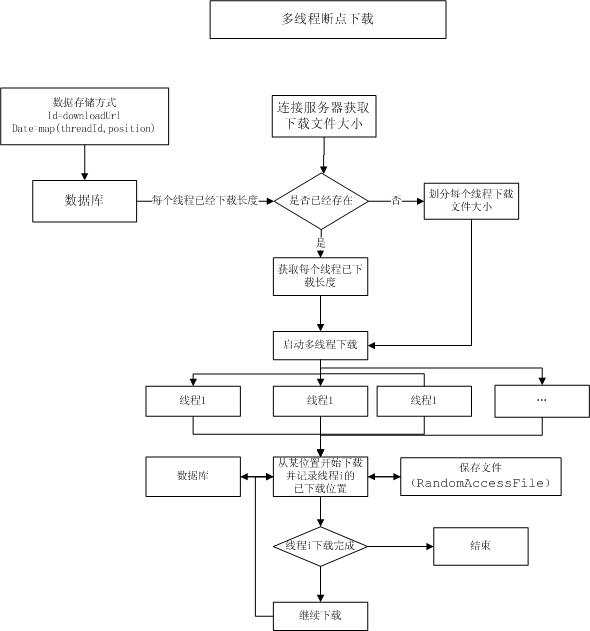
\includegraphics[width=130mm]{./figures/duandian.jpg}
  \caption{断点续传下载实现}
\end{figure}
本系统提供web端和安卓进行文件上传。

\par 安卓可以选择特定目录文件、及时拍照图片、最近修改图片进行上传。同时服务器会对上传文件加锁,如果上传的过程中
用一个并发的线程上传相同路径下的相同文件名文件,那么改线程就会陷入等待轮询状态。如果发现上传的文件有相同文件名,
那么就会提示是否覆盖,如果用户选择不覆盖原有文件,系统会为新文件添加序列号来保证相同路径下文件名的唯一性。
\begin{figure}[H]
    \centering
    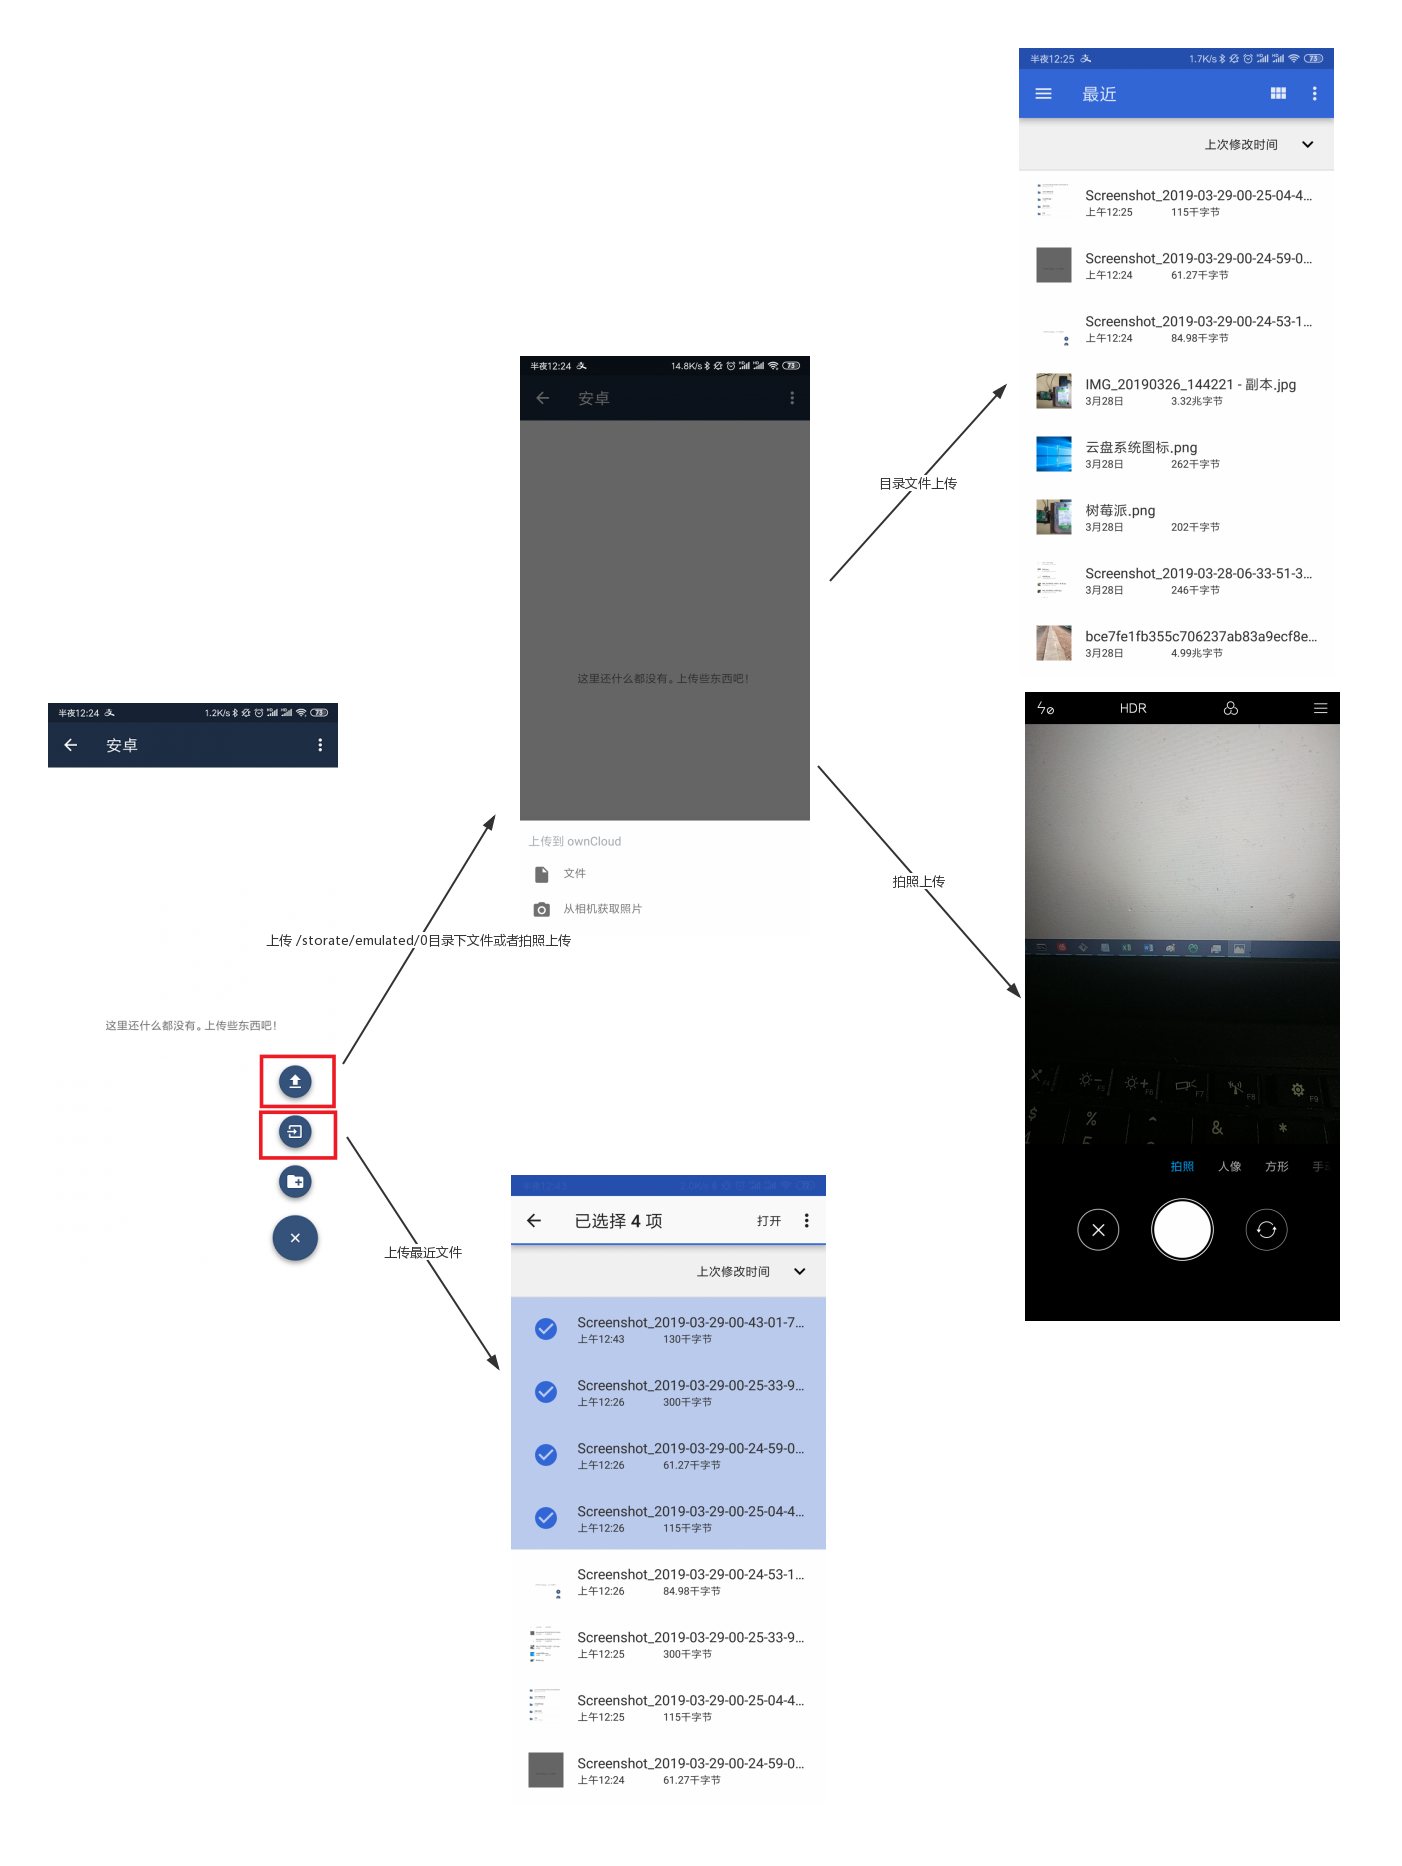
\includegraphics[width=130mm]{./figures/android_file_upload.png}
    \caption{安卓文件上传}
  \end{figure}
\subsubsection{文件下载}
\begin{figure}[H]
    \centering
    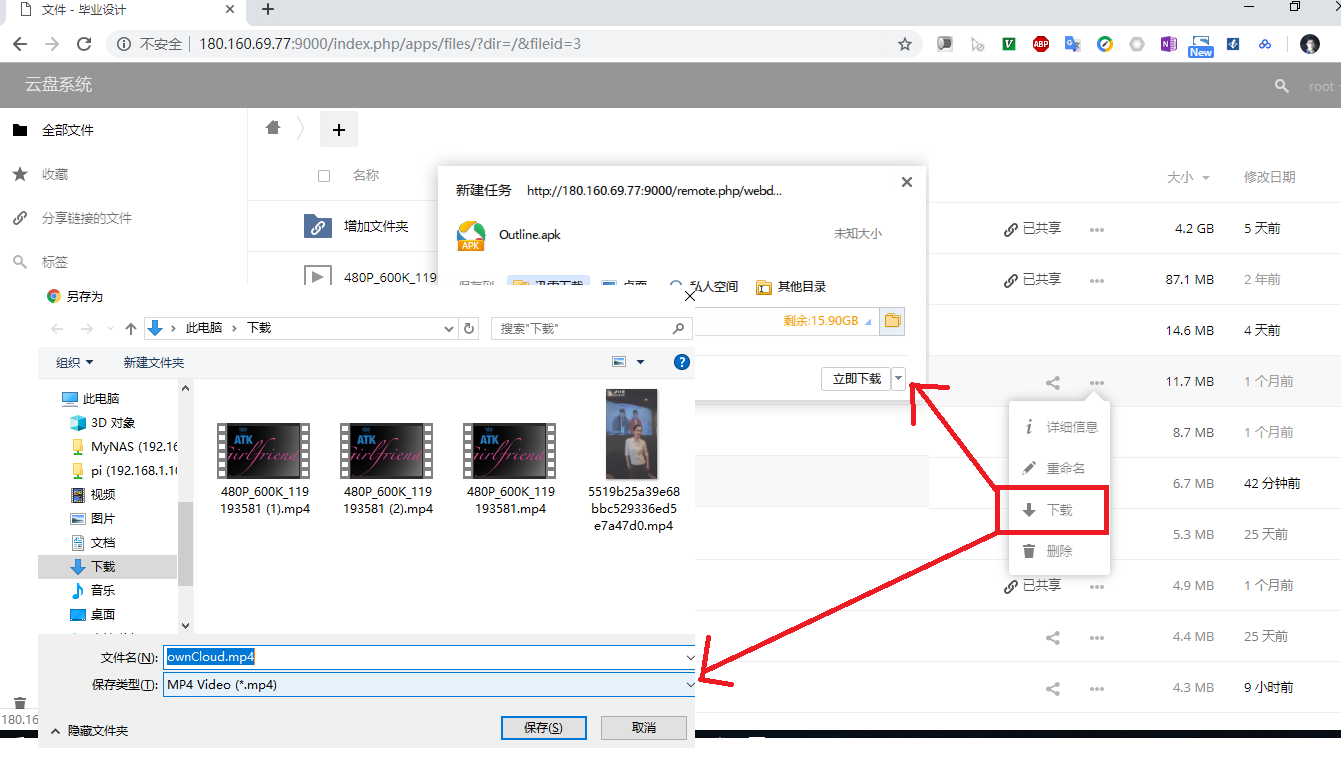
\includegraphics[width=130mm]{./figures/web_file_download.png}
    \caption{网页文件下载}
  \end{figure}

\subsubsection{视频播放}web端和Android端都支持视频播放功能,用户可以在线观看视频,web端视频播放器基于html5的videos标签,可以直接访问在apache
上的静态资源,省去了搭建流媒体服务器的麻烦。
\begin{figure}[htbp]
  \centering
  \subfigure[web在线视频播放器]{
  \begin{minipage}[t]{0.75\linewidth}
  \centering
  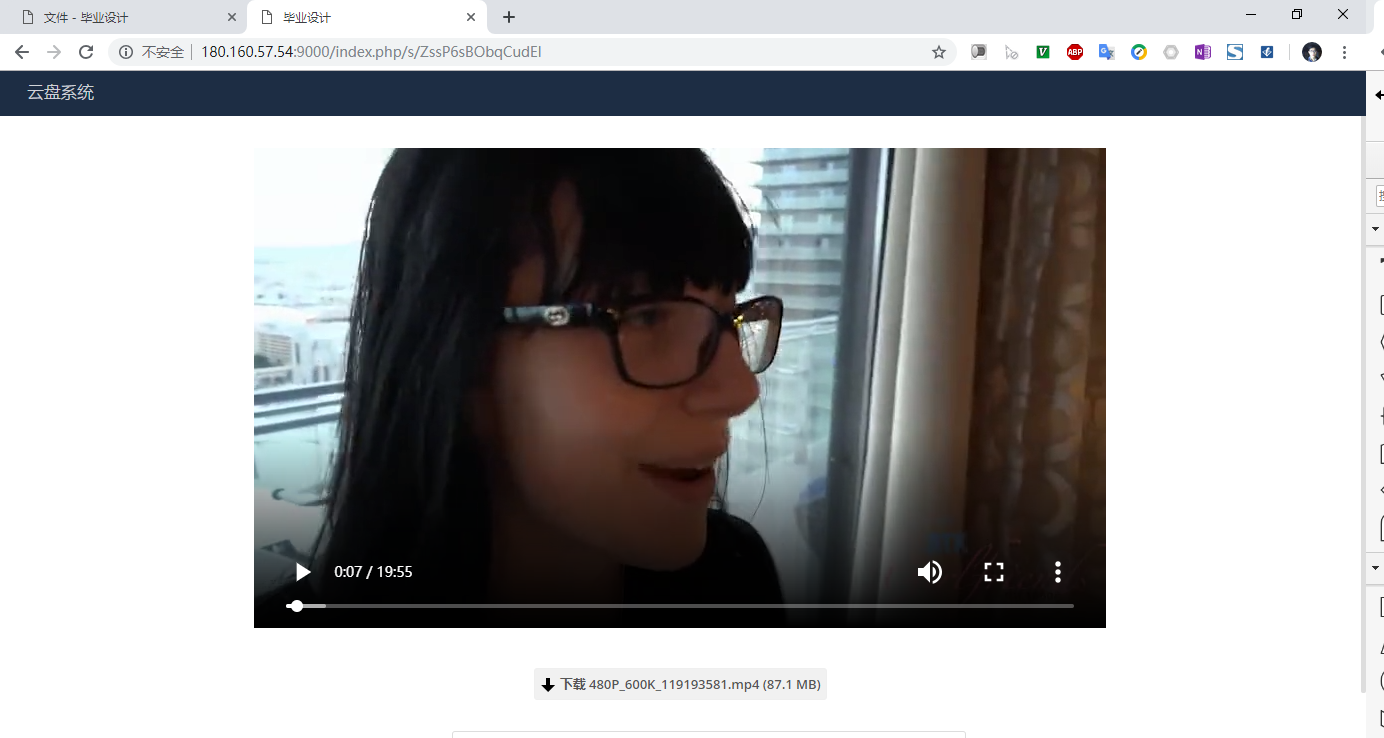
\includegraphics[width=98mm]{./figures/web_videos.png}
  %\caption{fig1}
  \end{minipage}%
  }%
  \subfigure[Android在线视频播放器]{
  \begin{minipage}[t]{0.25\linewidth}
  \centering
  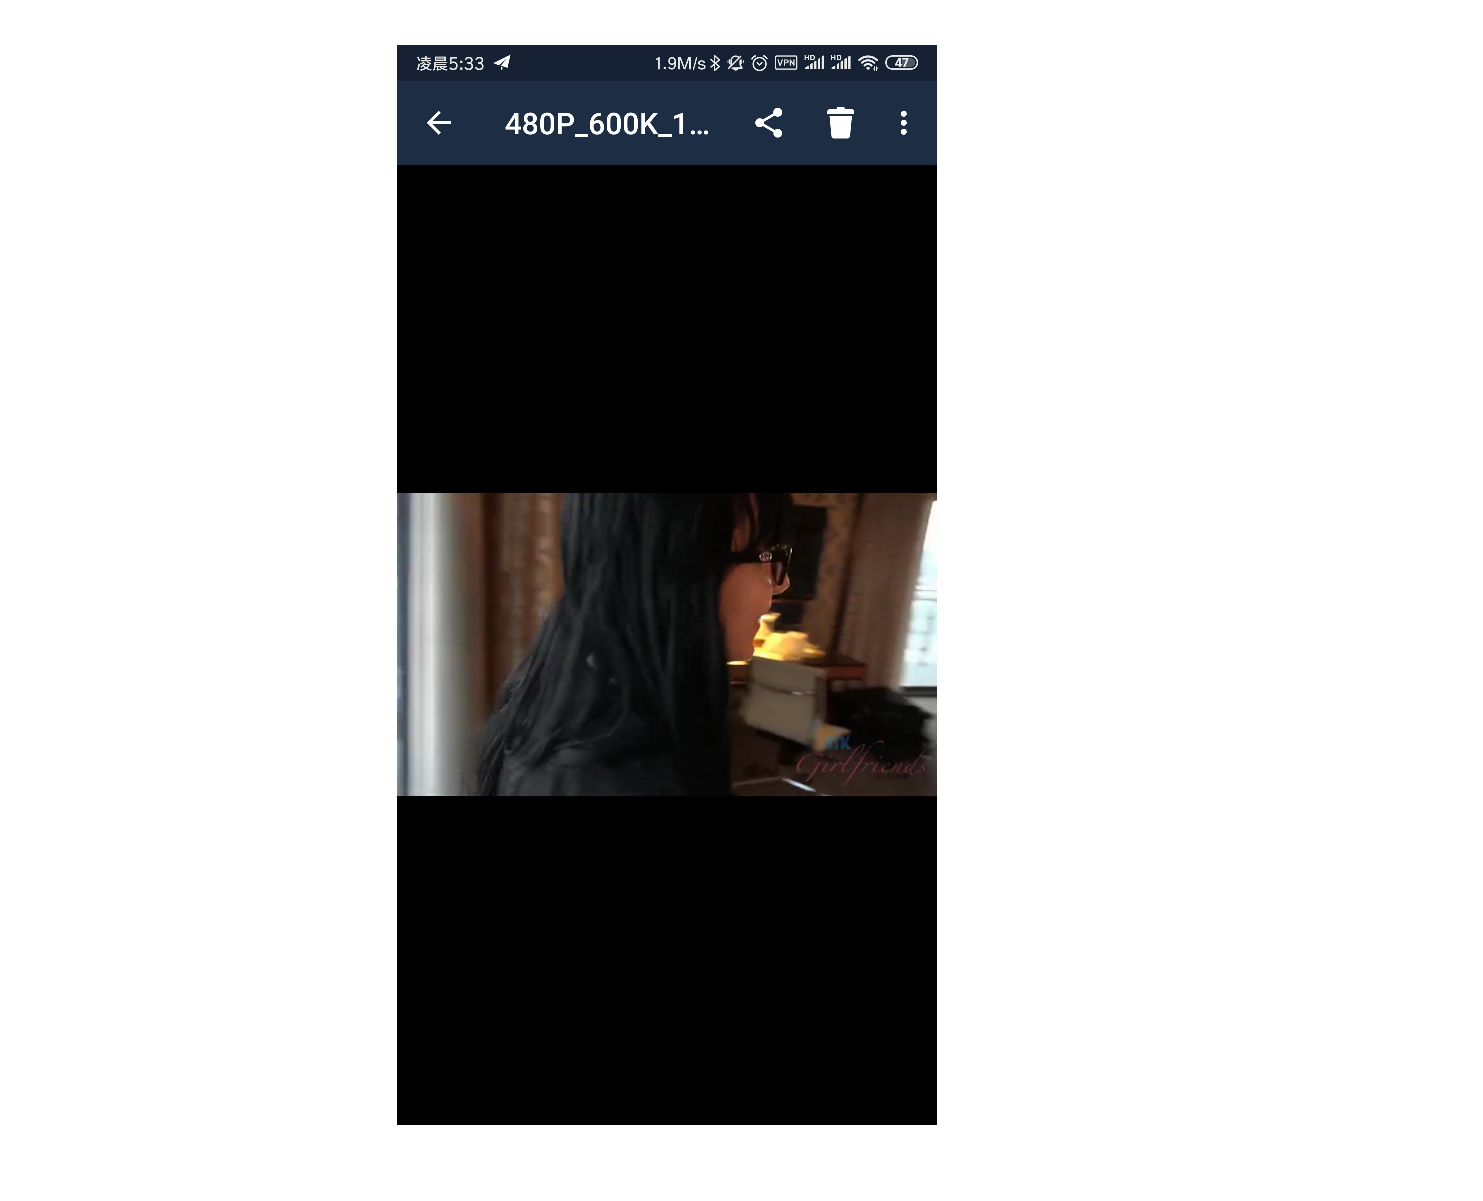
\includegraphics[width=32mm]{./figures/android_videos.png}
  %\caption{fig2}
  \end{minipage}%
  }%
  \centering
  \caption{视频播放}
  \end{figure}
  
\subsubsection{文件分享}
用户点击创建公共链接,客户端发送请求给服务器,服务器首先判断公共链接是否已经创建,如果已经创建,则返回已创建链接,
否则,利用php的shuffle随机函数根据文件uuid生成随机字符存入数据库并返回客户端。客户单端根据返回信息对连接名称,
分享密码,过期时间进行初始化,用户可以修改链接名称、密码、过期日期等信息,发送回服务器,服务器将请求参数持久化到mysql
数据库。

生成分享连接后,用户可以手动复制,通过社交软件或者邮件分享给互联网上的所有用户。安卓端有提供分享接口,通过实现
系统接口可以调用包括QQ、微信、短信、电子邮件或者其他第三发应用进行文件分享。
\begin{figure}[H]
    \centering
    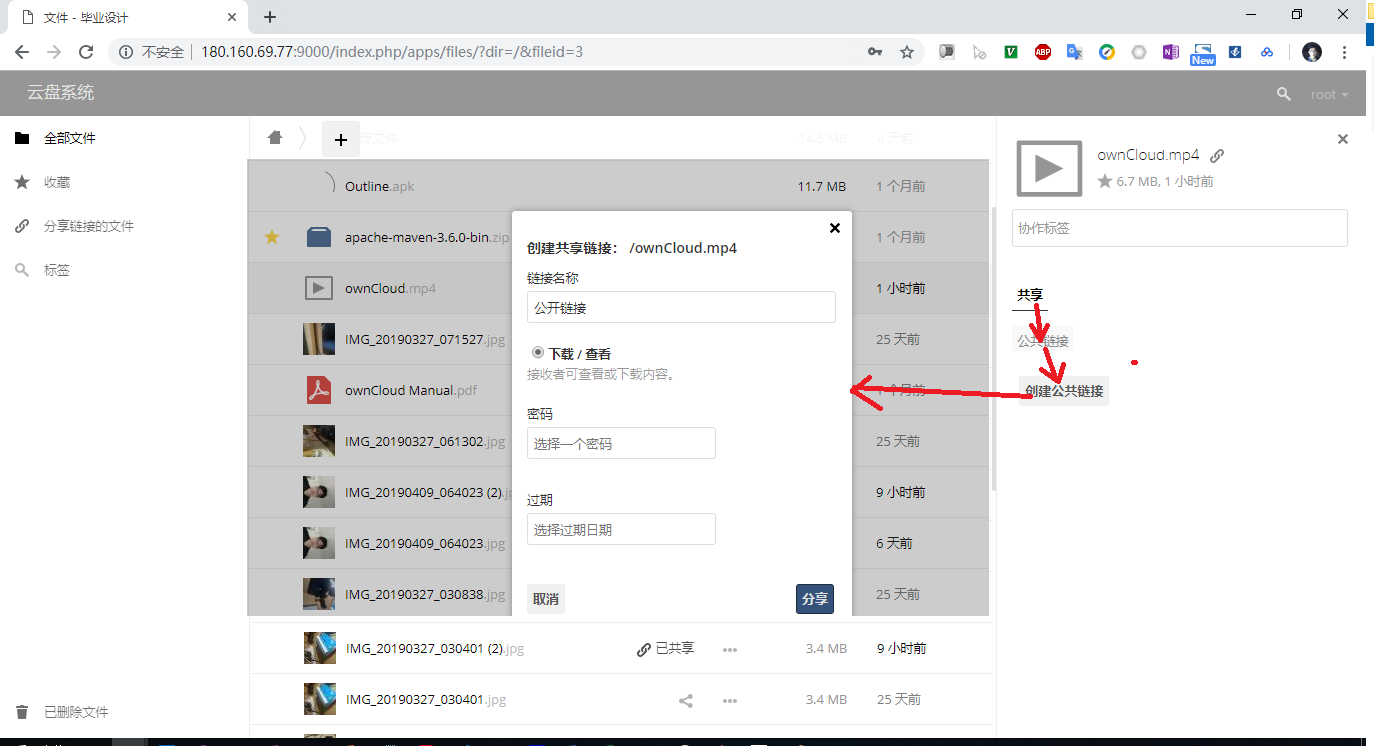
\includegraphics[width=130mm]{./figures/web_file_share_1.png}
    \caption{web分享文件}
    \label{android_videos}
  \end{figure}
\begin{figure}[H]
\centering
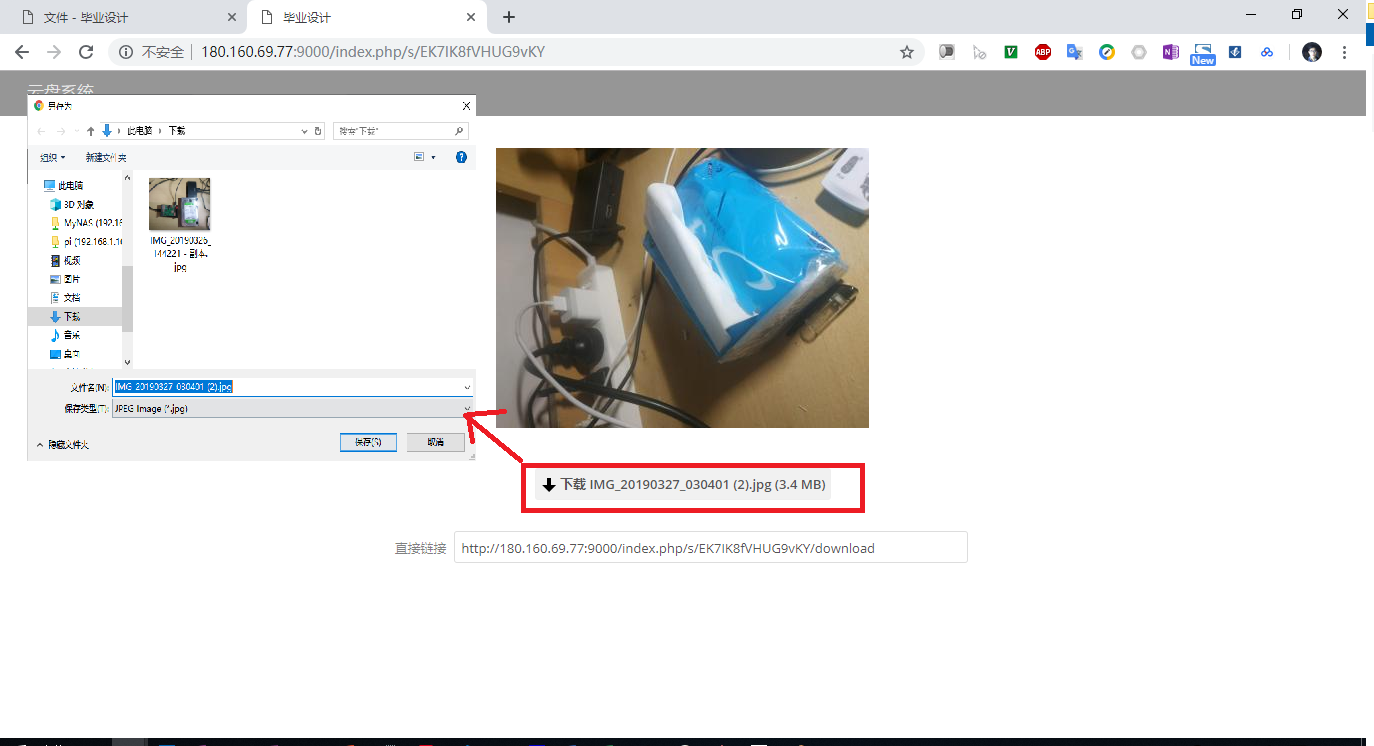
\includegraphics[width=130mm]{./figures/web_file_share_2.png}
\caption{web端访问分享文件}
\label{android_videos}
\end{figure}

\begin{figure}[H]
    \centering
    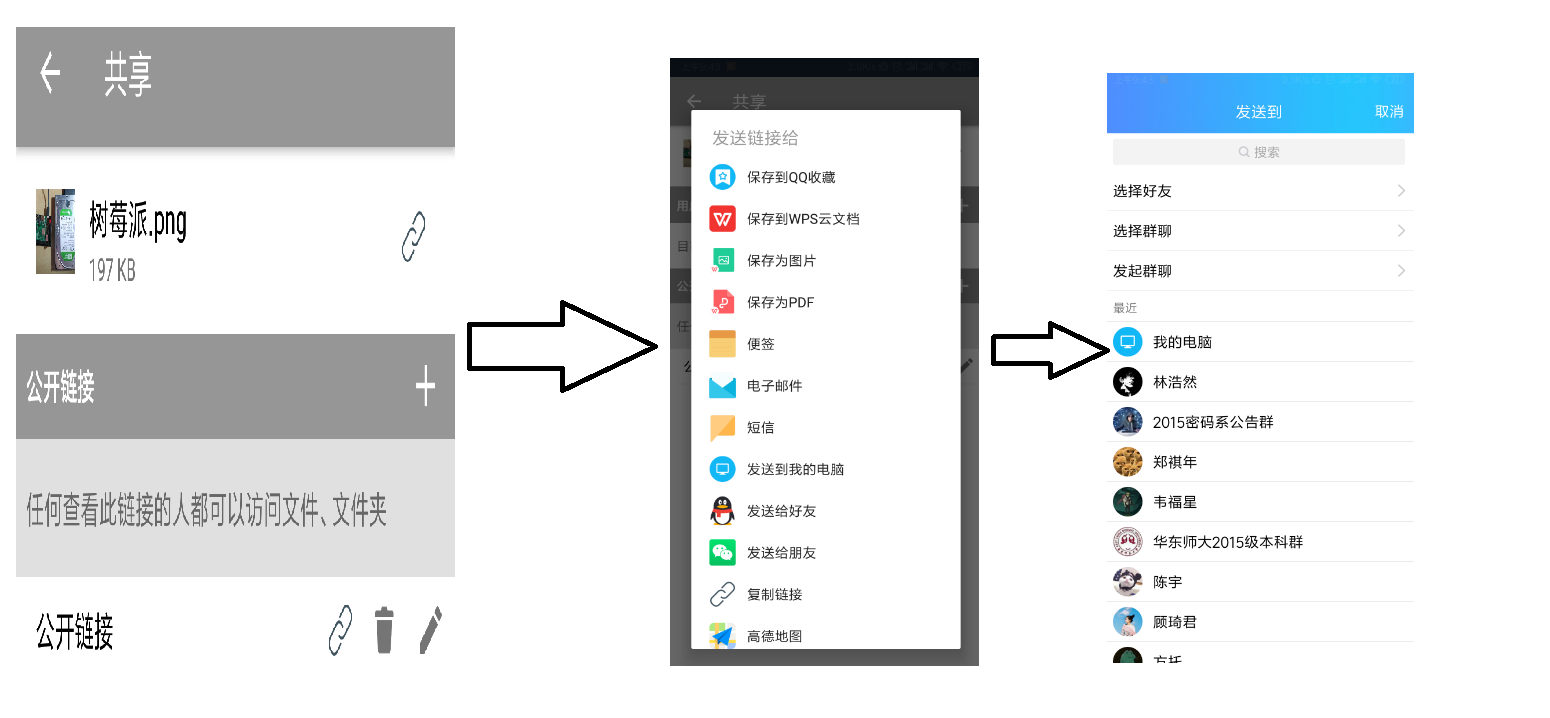
\includegraphics[width=130mm]{./figures/android_file_share.png}
    \caption{安卓端分享文件}
    \label{android_videos}
  \end{figure}

\subsubsection{手机文件自动备份}
安卓客户端默认不提供自动备份功能,因为自动备份的实现是安卓客户端会在后台开启一个backup的service线程,然后
以固定的时间轮询查看备份目录是否用新文件增加,如果用增加,service会调用volley网络请求工具上传文件给服务器,
并在本地保存上传快照。

用户也可以选择是仅上传图片、仅上传视频、仅WiFi网络条件下上传、上传文件后是否保留原文件等设置项。
\begin{figure}[H]
    \centering
    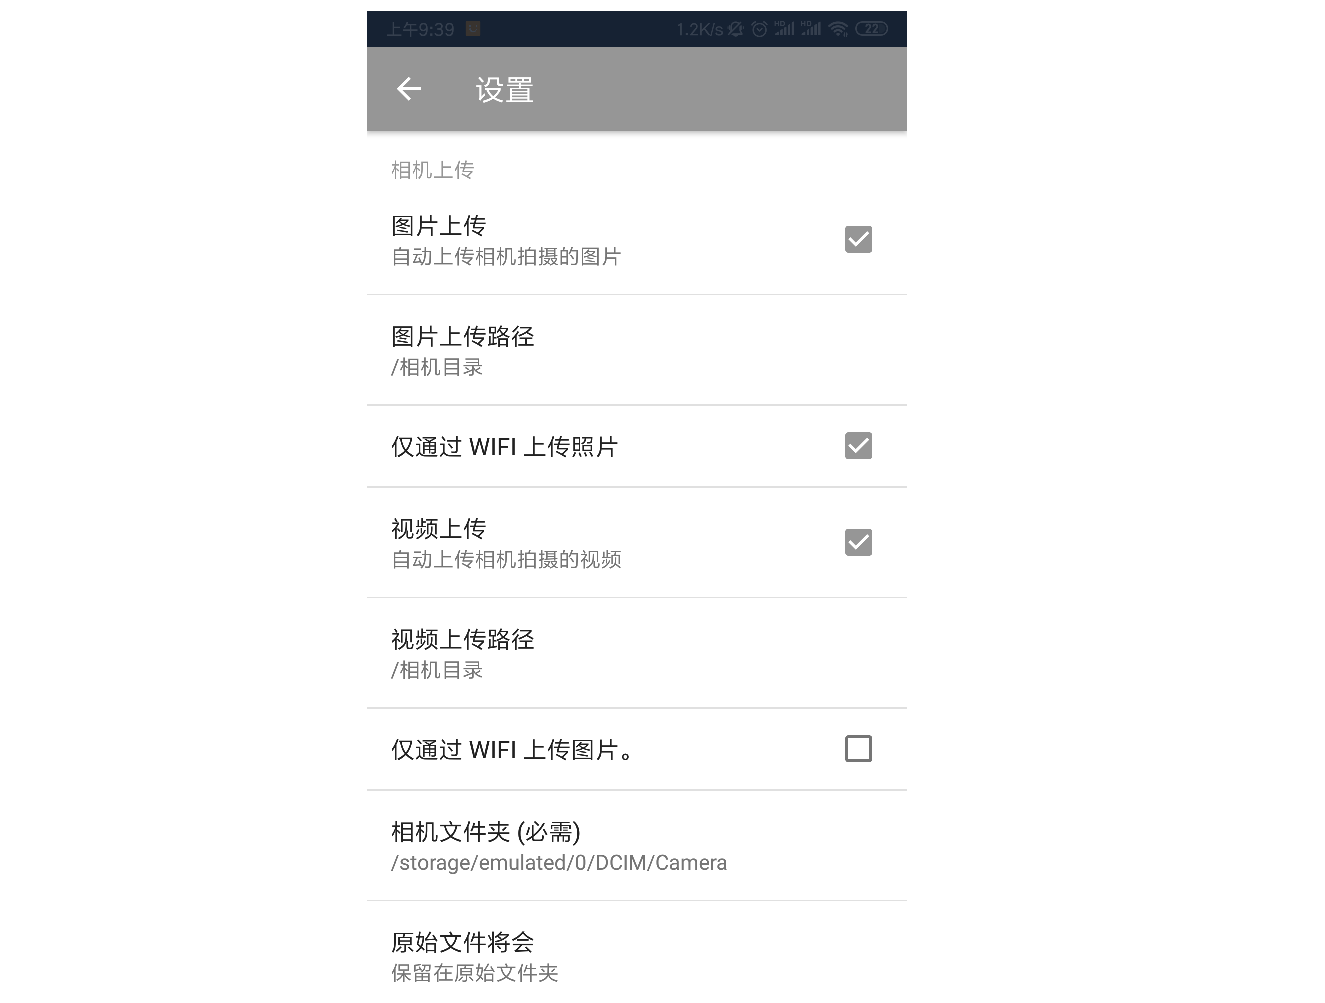
\includegraphics[width=130mm]{./figures/android_file_bck.png}
    \caption{安卓端文件备份设置}
    \label{android_videos}
  \end{figure}

\subsubsection{文件收藏、标签、搜索、已删除文件分类实现}
系统会将文件分为全部文件、收藏、分享文件、已删除文件四大类,用户可以根据自己的需求为文件分类或者打标签,
在web客户端会提供不通文件类型的入口,极大方便了用户查找文件。

实现的原理是创建四张文件表,用户在为文件归类时会往数据表中写入数据,所有文件默认时全部文件类型。当用户进入不同
的文件入口时,服务器会各自查询MySQL中的数据表,返回结果会客户端。
\begin{figure}[H]
    \centering
    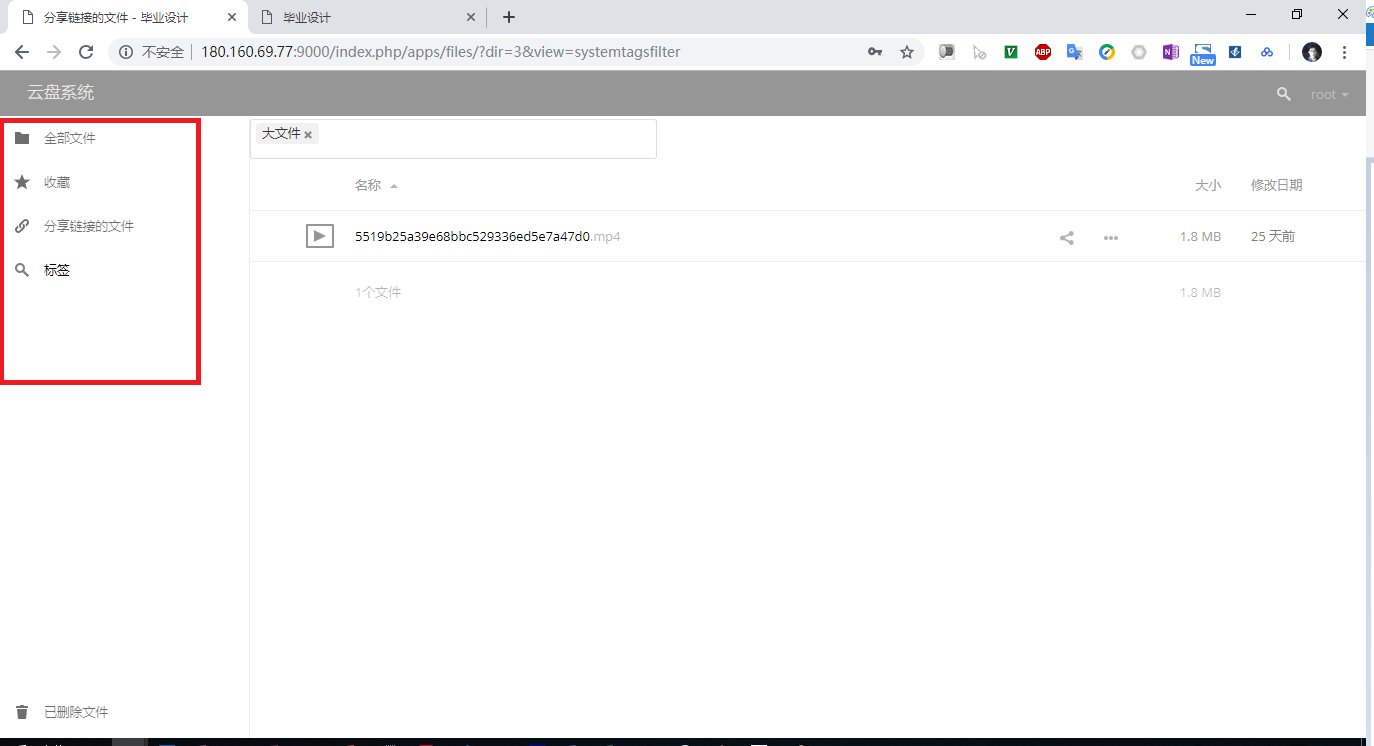
\includegraphics[width=130mm]{./figures/web_file_attach.png}
    \caption{安卓端文件备份设置}
    \label{android_videos}s
  \end{figure}

\subsubsection{文件增量备份、异地备份实现}
Merkle树是一种基于哈希的数据结构。 Merkle树是树状数据结构,其中树中的每个叶节点是数据块,
并且每个非叶节点是其子节点组合的散列。 通常,Merkle树是二叉树,这意味着Merkle树中的每个节点都有两
个子节点。 当然,Merkle树可以是多叉树,例如以太坊平台。 为简单起见,我们将在本文中仅讨论二进制Merkle树。

Merkle树广泛用于分布式系统中进行数据验证\cite{r20,r21}。 通常在分布式系统中,由于我们将数据存储在许多不同的机器上,
因此数据验证对于确保数据的可靠性和一致性尤为重要。 例如,如果我们更新机器上的一段数据,
则必须将更新传递给分布式系统中的所有机器以确保数据的最终一致性,以便比较不同机器上的数据。
\begin{figure}[H]
    \centering
    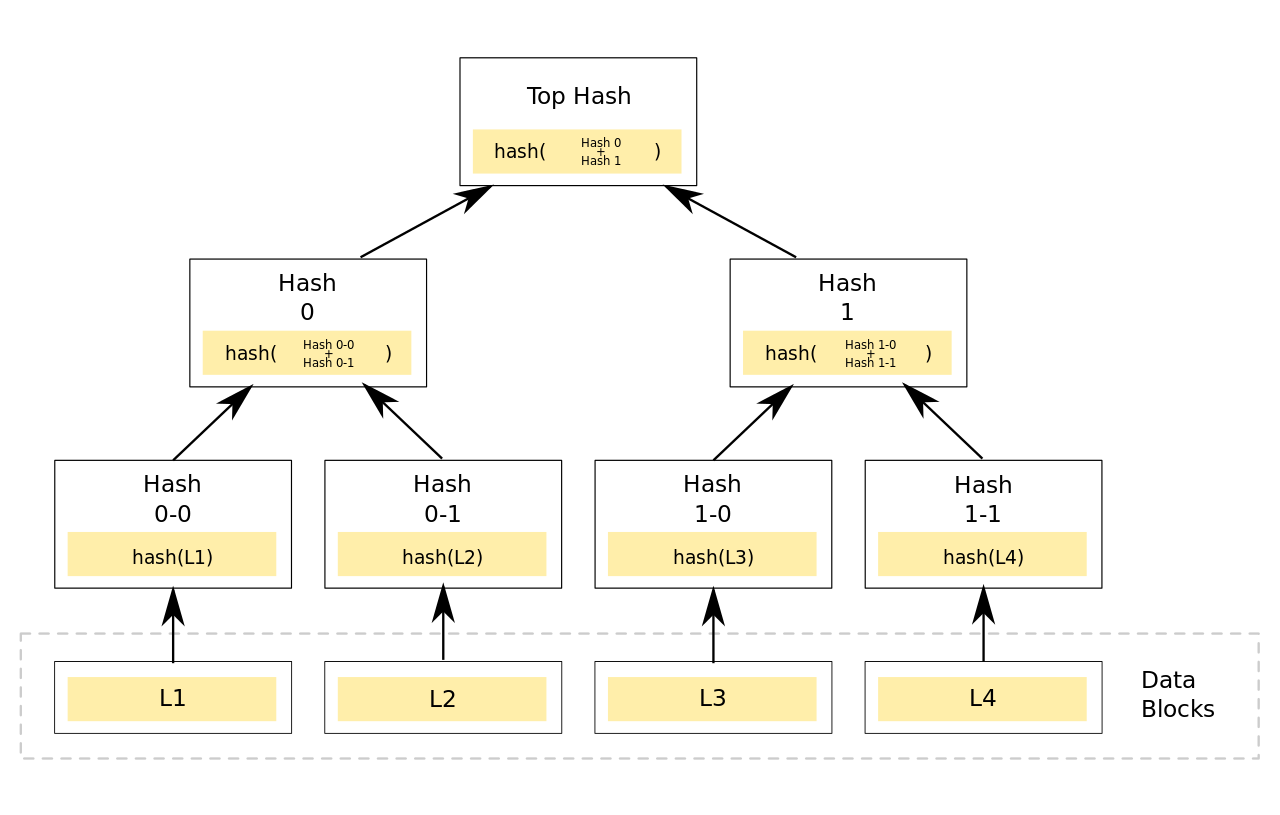
\includegraphics[width=130mm]{./figures/merkle_tree.png}
    \caption{Merkel树}
    \label{android_videos}s
  \end{figure}

本系统至少需要两台服务器进行数据备份,服务器间的数据必须保持同步。 如果数据不一致,则必须快速定位不一致的节点。
本系统为每台机器上的每个目录实现Merkle树,以便在比较两台机器之间的数据时,可以从Merkle树
根节点开始比较。 如果根节点相同,则表示两个副本当前一致,不再需要任何处理; 如果不一致,则遍历Merkle树,
可以快速定位到不一致的节点进行备份。相比于无脑地对文件进行完全备份,使用文件的哈希值作为文件的身份标识来
构建Merkle树的做法提升了备份的速度和存储空间

文件备份流程
\par (1) A服务器向B服务器发送需要与Merkle树的根节点对应的哈希值。
\par (2) B服务器接收此值并将其与正在构建的Merkle树的根节点哈希进行比较。
\par (3) 如果两个值相同,则表示两者存储的文件相同。
\par (4) 否则,B服务器需要像A服务器那样的哈希值来请求与根节点对应的两个子节点。
\par (5) A服务器将相应的值发送给B服务器。
\par (6) B服务器比较相应节点中的散列值,并重复步骤4和5,直到B服务器找到导致不同散列值的一个或多个数据块。
                             %
\section{系统测试}
无论是软件开发完成后还是开发的过程中,验证需求,寻找bug都是不可避免的工作。一个软件系统需要通过专业测试工作,全面的对需求进行正确性验证,找出隐藏的bug,并加以修复,才可以交付到用户手中使用。一个不经过测试的项目部署到生产环境中,出现影响用户体验甚至导致用户数据丢失、遭受黑客攻击等严重后果的概率很难被忽视。本章将对本人的测试工作进行详细的介绍,包括测试环境的搭建、测试计划、测试用例设计、测试执行以及测试结果数据的收集与评估等内容\cite{r31}。
\subsection{测试方法}
软件测试方法主要需要验证系统的可靠性和故障恢复力、负载能力,抗压能力和并发性等。
软件测试方法主要对系统的基本性能和服务器负载能力,服务器抗压性程序并发等情况进行测试,这需要验证系统的可靠性和失效恢复等功能,
在系统测试阶段,除了传统的功能测试之外,还需要额外的系统测试来测试无线网络环境的性能和并发多任务处理性能。
测试人员必须遵循测试要求,制定相应的测试方法和策略,创建相应的测试环境,并开发特定的测试用例。
\paragraph{黑盒测试}
黑盒测试也称为功能测试,测试系统功能是否能正常使用,黑盒测试可以说是最基本的测试。在测试中,测试人员可以
不需要理解功能的实现细节、内部代码结构和内部特征,最直观的解释是就是点点鼠标,等待结果是否符合预期。
它仅根据要求测试文档规范检查程序功能是否正常使用,也是测试项目的最开始的阶段,一般开发人员会在开发的过程中做一些简单的黑盒测试来验证
代码的一般最低标准的正确性。黑盒测试侧重于程序的外部结构,无论内部逻辑结构如何,主要测试软件接口和软件功能。黑盒测试是测试人员给出测试用例,
并根据用例输入相对应的数据和验证输出是否符合预期。显然,如果外部特征设计有问题或规格不正确,则无法找到黑盒测试方法。
黑盒测试可以帮助我们发现下面的几类错误:
\subparagraph{功能不正确或遗漏} 比如安卓端在登录注册的过程中需要在本地持久化JSESSIONID来作为身份令牌来保持登录状态,不同于web端浏览器会自动在Cookie中保存JSESSIONID,本系统的安卓端网络工具使用Retrofit2 + RxJava + Okhttp3,是没有自动化保存JSESSIONID的功能的,在后来的功能测试工作中发现了缺乏JSESSIONID造成的验证错误。
\subparagraph{界面错误} 比如Loaderunner在测试过程中会保存用户界面的html ui界面,可以通过Loderunner设置验证条件来验证界面页面元素的可用性,命名是否统一,界面中的文字是否正确,文字和图像组合是否完美,页面是否漂亮。
\subparagraph{输入和输出错误} 最常见的测试场景就是用户在操作一些表单数据的时候,比如用户在登录时,输入不存在用户名,过长的用户名,不正确的口令、只输入用户名或口令、恶意用户注入SQL代码,或者JavaScript代码等,
在这些过程中程序是否能给出人性化的错误提示都是要考量的一些方面。
\subparagraph{数据库访问错误}例如,攻击者通过常规网页将其SQL代码传递给应用程序。从而通过执行开发人员未预期的SQL代码,偷窃或者破坏数据库中的数据。当然开发这也可以通过限制访问数据库账号权限、参数化使用命令、调用存储过程等方法来避免SQL注入。
\subparagraph{性能错误}当存在大量并发方案和磁盘读写时,性能瓶颈是不可避免的。 例如,磁盘I / O性能,CPU性能和内存性能问题,分为网络瓶颈,服务器操作系统瓶颈,服务器硬件瓶颈和应用程序瓶颈。

\paragraph{压力测试}
软件压力测试是测试工作中一个非常重要的组成部分,一般在开发的初级阶段会做一些简单的功能测试,验证程序是否能正确跑起来,
但是如果没有做正规的压力测试的化,那么在生产环境中最非常容易出现问题,最常见的就是系统在处理并发场景是遇到的性能瓶颈,
常见的就是内存不足,数据库发生死锁等场景,如果没有在测试结果发现以上问题,那么在项目部署到生产环境上去之后就会遭受损失。
和功能测试比较依赖于手动测试相比,性能测试会比较依赖自动化的一些操作,测试人员会编写一些测试脚本对并发场景、混合场景进行模拟,
比较常见的性能测试工具是惠普的LoaderRunner,测试人员可以先手动点击一些功能项,LoaderRunner会将这些操作记录下来转化脚本,
测试人员只需要进行简单的配置最可以模拟并发场景、混合场景了。同时LoaderRunner会提供一些测试报告,大大提高了测试人员的工作效率。
性能测试主要对内部内存、CPU 可用性、磁盘空间和网络带宽这些方面进行测试。

\subsection{测试环境和测试工具}
本文需要特定的计算机硬件,软件,网络设备和日志数据平台来完成软件测试任务。 稳定和可控的测试环境有助于测试人员缩短完成测试用例所需
的时间,同时测试人员也不用额外费心设计测试用例和维护测试程序,并且可以保证所有提交的缺陷可以终准确无误的复现。

为了尽最大努力模拟真实情况,测试的过程是选择了寝室的局域网、校园网、无线蜂窝4G网络、北京上海城域网之间进行,测试用的硬件环境和软件环境、测试工具分别在下列三个表中列出。

下表是测试所需要的软件环境,包括Linux、Apache、Mysql、PHP、Chrome、Internet、Android 、Windows。
% \newpage
\begin{table}[htbp]\center
    \caption{软件环境(相关软件、操作系统等)}
    \begin{tabular}{lcccccl}
        \toprule
        名称 &  版本 & 数量 & 获得途径 \\
        \midrule
        Linux & Raspbian GNU/Linux 9 & 1 & https://www.raspberrypi.org/ \\
        Apache &  Apache/2.4.25 (Raspbian) & 1 & http://www.apache.org/ \\
        Mysql & mysql 5.7 & 1 & https://www.mysql.com/ \\
        PHP & PHP 7.0.33 & 1 & https://www.php.net/ \\
        Chrome & 73.0.3683.86(正式版本) (64 位) & 1 & https://www.google.com/chrome/ \\
        Internet Explower & IE 11.379.17763.0 & 1 & Windows系统自带 \\
        Android & MIUI 10/Android 9.0 & 2 & 手机厂商自带 \\
        Windows & windows 7/10 & 5 & 计算机厂商自带 \\
        \bottomrule 
    \end{tabular}
\end{table}
下表是测试所需要的硬件环境,包括TP-Link 路由器、Raspberry Pi、西部数据2T硬盘、计算机、移动手机\begin{table}[htbp]\center
    \caption{硬件环境(网络、设备等)}
    \begin{tabular}{lcccccl}
        \toprule
        名称 &  版本 & 数量 & 获得途径 \\
        \midrule
        TP-Link 路由器 & TL-WR886N & 1 & 自行购买 \\
        Raspberry Pi & Raspberry Pi 3 Model B+ & 1 & 自行购买 https://www.raspberrypi.org/products/ \\
        西部数据2T硬盘 & & 1 & 自行购买 \\
        计算机 & Thinkpad x260 / DELL台式机  & 2 & 自行购买/公共财产 \\
        移动手机 & 小米  华为 & 2 & 自行购买 \\
        \bottomrule 
    \end{tabular}
\end{table}
下表是测试所需要的压力测试工具,Web端使用loadrunner,安卓端用到了Appium,使用抓包工具Wireshark进行网络数据包分析。
\begin{table}[htbp]\center
    \caption{测试工具}
    \begin{tabular}{lcccccl}
        \toprule
        名称 &  版本 & 数量 & 获得途径 \\
        \midrule
        Appium & V1.8.1 & 1 & 	通过网络下载 \\
        Loaderunner & 3.141.59 & 1 & 通过网络下载 \\
        Wireshark & 3.0.0 & 1 & 通过网络下载 \\
        \bottomrule 
    \end{tabular}
\end{table}

\subsection{系统功能测试}
在明确系统的测试目标之后可以根据测试目标制定合理的测试计划。就本云盘系统来说,测试目的主要包括系统实现是否满足云存储需求、性能是否足够稳定、以及安全性是否可靠三个方面。
\begin{table}[hp]\center
    \caption{用户登录功能测试}
    \begin{tabular}{p{2cm}p{5.5cm}p{5.5cm}p{1cm}}
        \toprule
        测试项 &  操作步骤 & 预期结果 & 结果 \\
        \midrule    
        正确输入            & 在登录框输入正确的用户名和口令,回车或点击登录按钮  & 登录成功后,web端跳转到index.php/apps/files页,安卓端会跳转到APPActivity页面 & 通过 \\                                        
        错误输入            & 在登录框输入错误的用户名口令,回车或点击登录按钮 & 提示登录失败,提供修改口令链接 & 通过 \\
        用户注册            & 在登录框输入未注册用户,提示请先注册,然后进行登录      & 提示登录失败,提供注册链接,注册成功后成功跳转 & 通过 \\
        用户注销提示        & 在登录框输入已经注销的用户,回车或点击登录按钮 & 提示用户不存在或口令错误,提供修改口令或注册用户链接 & 暂未实现 \\
        口令显示            & 在登录框输入口令 & 安卓端和web端对明文口令进行隐藏显示 & 通过 \\
        特殊字符            & 在登录框用户名输入中文、特殊字符,回车或点击登录按钮  & 登录成功后,web端跳转到index.php/apps/files页,安卓端会跳转到APPActivity页面 & 通过 \\                                    
        字符串长度          & 在登录框输入长度为2,4,8,16,32,64,128,256长度用户名,回车或点击登录按钮 & 用户名在4~32长度之间允许向服务器发送验证请求,否则提示用户名过长或过短,如果用户自行构造登录请求,服务端验证后返回400Bad Request验证码 & 通过 \\
        口令特殊字符        & 在登录框输入中文,特殊字符口令,回车或点击登录按钮 & 提示口令不支持该格式,用户不能发送请求,如果用户自行构造登录请求,服务端验证后返回400Bad Request验证码 & 通过 \\
        口令长度            & 在登录框输入长度为2,4,8,16,32,64,128,256长度口令,回车或点击登录按钮 & 口令长度在4-16之间用户可以发送请求,其余范围提示口令过长或过短,用户不能发送请求,如果用户自行构造登录请求,服务端验证后返回400Bad Request验证码 & 通过 \\
        口令大小写          & 在登录框分别输入大小写格式口令,回车或点击登录按钮 & 系统对口令大小写敏感,服务器使用md5对明文口令进行hash生成128位散列值,口令大小写不同会生成不通的散列值,和数据库口令进行比较返回验证结果 & 通过 \\
        常见口令            & 在登录框输入一些简单常用字符串口令,回车或点击登录按钮 & 登录成功后,web端跳转到index.php/apps/files页,安卓端会跳转到APPActivity页面 & 通过 \\                                   
        口令加密存储        & 登录注册成功后查看数据库口令存储方式 & 系统将用户明文口令进行md5哈希后存入数据库 & 通过 \\
        \bottomrule 
        \label{user_login_function}
    \end{tabular}
\end{table}
\begin{table}[htbp]\center
    \caption{用户登录安全性测试}
    \begin{tabular}{p{2.5cm}p{5cm}p{5cm}p{1cm}}
        \toprule
        测试项 &  操作步骤 & 预期结果 & 结果 \\
        \midrule
        验证拦截 & 不登录状态,在浏览器地址栏直接输入需要登陆后地址、通过Http请求的工具Postman发送登陆后地址请求 & 服务器会对请求地址请求进行拦截,返回302状态码和重定向地址http://180.160.68.247:9000/index.php/login?redirecturl=请求地址 & 通过 \\
        Cookie httponly & web端通过js代码获取浏览器Cookie值,安卓端通过wireshark对app请求进行截获,察看Cookie请求头 & js无法获取Cookie值,wireshark无法查看Cookie值 & 失败 \\
        用户名和口令加密 & 通过wireshark对用户登录请求进行截获,查看用户名和口令是否通过加密的方式发送给Web服务器  & 用户的用户名和口令都得到加密,wireshark看到的是加密后的密文 & 未实现 \\
        前后端协同验证 & 在前端用js验证输入参数是否符合规范,后端也需要验证  & 前后端都进行参数验证,既能保障普通用户输入的正确性,也能防止黑客进行恶意攻击 & 通过 \\
        SQL注入 & 通过SQL注入脚本工具在登录框构造SQL语句,比如万能登录SQL语句、删除表数据SQL语句 & 前后端都有进行输入验证,屏蔽SQL 注入攻击,服务端验证后返回400Bad Request验证码  & 通过 \\
        XSS攻击& 通过XSS攻击脚本工具在登录框构js代码,读取、篡改、添加、删除用户敏感数据 & 进行Token验证、Referer验证、隐藏令牌等措施,防御XSS攻击 & 未实现 \\
        登录次数限制 & 通过python requests库对用户名和口令发动穷举攻击 & 服务器对单一ip地址的登录请求次数进行限制,登录次数超过5次会对该用户进行登录限制,5小时内不能再进行登录,对于频繁发送请求进行dos攻击的ip地址加入黑名单,返回401 状态码 & 通过 \\
        多用户单机器登录 & 在一台计算机或者移动终端上登录多个用户 & 用户可以通过浏览器的无痕模式进行单机器多用户登录,并且服务器会根据不通的sessionid返回对应的用户资源。安卓端可以通过app分身功能同时登录多个用户,服务器会根据不通的sessionid返回对应的用户资源 & 通过 \\
        单用户多机器登录 & 在web和移动app上同时登录 & 服务器会根据sessionid在后端保存登录用户信息用户可以在在web和移动app上同时登录 & 通过 \\
        验证次数限制 & 用户连续输入三次错误口令 & 用户一段时间内不允许登录,超出时间后能够继续登录 & 通过 \\
        session日期 & 关闭浏览器、或者卸载重装app、超过24小时发送访问资源请求 & session无效后用户无法访问系统资源 & 通过 \\
        输入方式 & 在用户名和口令输入框撤销、复制、粘贴文本 & 支持用户快捷键操作,比如撤销、复制、粘贴等操作 & 通过 \\
        用户同时登录 & web和app同时登录,同时上传下载文件 & 是允许同名用户同时登录进行操作,但是对文件进行加锁机制,保证事务的一致性,原子性 & 通过 \\
        网络判断 & 在断网条件下使用app客户端、web客户端,在恶劣网络条件下使用app客户端、web客户端 & 有未联网和网速较慢提示 & 通过 \\
        \bottomrule 
    \label{security_user}
    \end{tabular}
\end{table}
\begin{table}[htbp]\center
    \caption{文件上传下载测试表}
    \begin{tabular}{p{4cm}p{5.5cm}p{2.5cm}p{1cm}}
        \toprule
        测试项 &  操作步骤 & 预期结果 & 结果 \\
        \midrule
        命名检查& 分别构造长度、后缀名符合或不符合规范的文件进行上传。 & 符合规范上传成功,否则失败 & 通过 \\
        类型检查& 上传所有类型文件、二进制文件、可执行文件、文本文件等等。 & 所有文件上传成功。 & 通过 \\
        空文件上传 & 选择一个空文件,进行上传。 & 文件上传失败。 & 通过 \\
        正常小文件上传 & 分别选择128KB、1MB、5MB、50MB大小文件上传 & 文件上传成功。 & 通过 \\
        正常大文件上传 & 分别选择100MB、200MB、500MB、1GB、2GB、4GB、5GB大小文件上传 & 文件上传成功。 & 通过 \\
        超大文件上传 & 选择6GM大小文件上传如进行上传。 & 文件上传失败。 & 通过 \\
        正常小文件下载 & 分别选择128KB、1MB、5MB、50MB大小文件下载 & 文件下成功。 & 通过 \\
        正常大文件下载 & 分别选择100MB、200MB、500MB、1GB、2GB、4GB、5GB大小文件下载 & 文件下成功。 & 通过 \\
        上传下载响应时间 & 分别上传或者下载文件,测试响应时间 & 响应时间在2s以下 & 通过 \\
        \bottomrule 
    \end{tabular}
\end{table}

\subsubsection{用户登录功能测试}
用户登录功能是否能实现是保证本系统是否能正常使用的前提,因此在开发本云盘系统的时候,用户登录模块不仅仅是用户输入用户名和口令,
在后台做验证,返回结果就行,而且背后的实现考量的因素很多,因为作为最基本的系统功能,同时还要考虑到安全性,
在开发的过程中就很不容易了。因此如表\ref{user_login_function}所示,本文在正确输入、错误输入、用户注册、用户注销提示、口令显示、特殊字符、字符串长度、口令
特殊字符、口令长度、口令大小写、常见口令、口令加密存储12个功能做了登录的功能测试。

测试结果表明,以上12个功能均已实现,用户在登录会有输入检测和结果提示,同时系统也对一些用户的输入进行验证,一定程度上保证了系统的安全性。

\subsubsection{用户登录安全性测试}
登录的安全性测试不同于登录功能上的一些验证,要验证登录功能是否在有一定的安全措施,需要理解功能实现的背后逻辑。安全测试
需要用到Wireshark抓取请求包,分析http报文是否会泄露表单数据,比如用户名和口令在表单中是否以明文形式存储;同时要查看
系统后台是否对口令进行哈希处理也需要在数据库查询,还有在实现单机单用户多机登录服务器的不同的sessionid的session中是否
持有相同的用户信息,这些需要在后台打断点调试才能知道结果。如表\ref{security_user}所示,本文分别在验证拦截、Cookie 
httponly、用户名和口令加密、前后端协同验证、SQL注入、XSS攻击、登录次数限制、多用户单机器登录、单用户多机器登录、验证
次数限制、session日期、输入方式、用户同时登录、网络判断14个进行验证。

测试结果表明,系统在XSS攻击、传输报文加密两个方面还存在欠缺,但是在其余安全措施方面均能达到预期目标。

\subsubsection{文件传输测试}
本系统的核心是为用户提供文件上传和下载的功能,整个系统的性能表现取决于树莓派作为功能承载的硬件,树莓派的网卡速率能达到500Mb/s,
同时在寝室的路由器也是500M网卡,实际测试下来在局域网能保证2.5MB/s的上行下载速度,在外网的环境下能保证500KB/s的上行下载速度,
也比较符合中国电信的20Mb宽带套餐,因此传输速度方面实在是没有可以更多方面的工作的介绍,不同于集群的工作能力,本系统所能达到的
性能表现只取决于树莓派的单机性能表现。同时在功能测试方面,本文分别对命名检查、类型检查、空文件上传、正常小文件上传、正常大文件上传、
超大文件上传、正常小文件下载、正常大文件下载、上传下载响应时间9个方面进行测试,测试结果表明系统功能能达到设计目标。

\subsubsection{性能测试}
同在Linux系统中可以使用dstat监视系统资源利用率,在性能测试为2个并发用户在下载大型文件的场景下,如图\ref{dstat}所示,树莓的cpu
利用率达到36%~54%的水平,磁盘的读速度维持在40MB/S的速度,网络速度能保持在1500KB/s的上行速度和5000B/S到9000B/s的下载速度。
就直观感受来说,基本可以满足2个并发用户的上传、下载、分享、搜索文件的需求。
\begin{figure}[H]
  \centering
  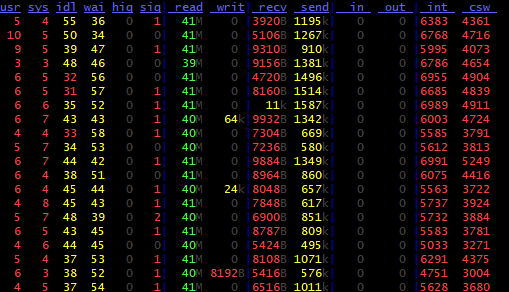
\includegraphics[width=130mm]{./figures/dstat.png}
  \caption{树莓派系统资源监视}
  \label{dstat}
\end{figure}
\newpage                             %
\section{总结和展望}
\subsection{研究和工作总结}
本系统是利用闲置的家庭宽带和淘汰的硬盘资源,在基于廉价的通用小型计算机树莓派(英语:Raspberry Pi)
的基础上开发出一个为用户提供文件的备份、共享、存储、访问、搜索、管理等功能,满足多终端访问的在线云盘存储系统。

本文的前期工作是收集市场上的云盘服务的定价、访问速度、系统稳定性和树莓派单片机配置、定价的等数据信息,通过比较价格,安全可
用性等方面,来决定本云盘系统的是否存在开发实现的现实意义。通过数据分析,在和市场上商业的云盘服务比较之后,本系统在特定条件下存在
成本和性能上的优势。

本系统利用LAMP(Linux-Apache-MySQL-PHP)来进行开发系统后端服务器开发,同时提供web客户端和安卓客户端来进行文件的访问和备份。

本系统的web端在主流的浏览器Chrome、Edge、IE11、QQ浏览器、360安全浏览器、360极速浏览器、百度浏览器、opera浏览器、手机端的uc浏
览器、小米系统浏览器等浏览器都可以正常访问。在安卓客户端用户可以上传手机上的图片、照片、文本,可以设置自动备份来自动备份手机中的
文件。

基于树莓派和二手机械硬盘的云盘系统的开发在成本上具有巨大的成本优势,同时在特定网络条件下的文件访问备份效果不错,也是本文的特殊意义所在。
\subsection{展望}
本文实现的云盘系统虽然能够一定程度满足当前项目的需求,但是在易
用性、安全性和定制化方面仍然存在改进和提高。

易用性还需进一步改进。一个非计算机专业的用户要使用本系统,需要掌握在路由器网络端口配置、树莓派系统搭建、
LAMP环境搭建和使用、计算机网络知识、Linux磁盘挂载、一些基本Linux命令和vim文本编辑、Android程序编译等等专业
知识。因此如果需要将本文的云盘系统作为产品推广,需要将一些操纵进行封装,让用户脱离复杂的参数配置而直接一键安装使用。
如果仅仅提供源码和文档,我相信对于大部分用户,甚至是计算机专业的用户都会非常头痛,因此一个完善可直接使用
的软件环境是今后需要努力的方向。

安全性还需进一步改进。因为开发时间仓促,本系统的网络传输协议使用的是HTTP,我们知道HTTP是明文传输,因此很容易
遭遇中间人攻击,传输数据被窃听和数据内容篡改,虽然我系统的使用场景在寝室、家中的局域网内,遭受黑客攻击的
可能性微乎其微,但是本系统有提供外网访问功能,因此还是存在一定的安全风险,所以将系统从HTTP迁移到HTTPS也是
今后努力的方向。

定制化还需进一步改进。本系统提供了两种客户端Web和Android,但是有电脑用户更倾向于使用桌面的客户端
进行数据备份下载,市场上主流的云盘服务百度云就同时用户Web,手机端,桌面端的应用,
人们也有使用桌面软件的使用习惯,因此下一步的改进的方向是开发出桌面客户端和IOS应用,从而覆盖更广的用户。
当然本系统还有一些缺失的功能,比如动态分享、垃圾文件清理、通话记录备份、通信录备份、短信备份等功能还存在缺失,
因此今后功能的添加也是一个努力的方向。
                             %
%%%%%%%%%%%%%%%%%%%%%%%%%%%%%%%%%%%%%%%%%%%%%%%%%%%%%%%%%

% \theendnotes %尾注

\cleardoublepage
\phantomsection    
\printbibliography[title={\heiti \centerline{\zihao {-3}参考文献}} ] %生成参考文献
\addcontentsline{toc}{section}{参考文献}

% \begin{appendices}   
% \clearpage
% %\renewcommand{\thesection}{\chinese{section}}  %生成附录
% \apdx{实验数据}
23333333333333333333333333333333333333333

\apdx{调查结果}
23333333333333333333333333333333333333333
% \end{appendices}

\makeacknowledgement

\end{document}